\pdfoutput=1

\documentclass{l4proj}

%
% put any packages here
%

\usepackage{listings}
\usepackage{color}
\usepackage{float}
\usepackage{natbib}
\usepackage{url}
\usepackage{enumitem}

\definecolor{dkgreen}{rgb}{0,0.6,0}
\definecolor{gray}{rgb}{0.5,0.5,0.5}
\definecolor{mauve}{rgb}{0.58,0,0.82}

\lstset{
  language=Scala,
  aboveskip=3mm,
  belowskip=3mm,
  showstringspaces=false,
  columns=flexible,
  basicstyle={\small\ttfamily},
  numbers=none,
  numberstyle=\tiny\color{gray},
  keywordstyle=\color{blue},
  commentstyle=\color{dkgreen},
  stringstyle=\color{mauve},
  breaklines=true,
  breakatwhitespace=true,
  tabsize=2
}

\lstdefinelanguage{Ini}
{
    basicstyle=\ttfamily\small,
    columns=fullflexible,
    morecomment=[s][\color{Orchid}\bfseries]{[}{]},
    morecomment=[l]{\#},
    morecomment=[l]{;},
    commentstyle=\color{gray}\ttfamily,
    stringstyle=\color{mauve},
    numberstyle=\tiny\color{gray},
    morekeywords={},
    otherkeywords={=,:},
    keywordstyle={\color{blue}\bfseries}
}

\newcommand{\code}[1]{\texttt{#1}}

\begin{document}
\title{Who To Follow In Context}
\author{Darren Burns}
\date{\today}
\maketitle

\begin{abstract}

A large number of users of Twitter rely on the service to follow discussions relating to ongoing events. The ``Who To Follow In Context'' project assists these users in finding other Twitter users who have been recently discussing such events. In particular, this project introduces real-time, frequently updating suggestions of users which model the evolving nature of the events that these recommendations are being made for. By architecting and designing the project as a message-driven, reactive application, we are able to process incoming streams of social media data in real-time whilst retaining overall system responsiveness. After implementation of the design concluded, it was extensively evaluated using a series of questionnaires, user evaluations, and experiments. This evaluation suggested that users appreciate the problem areas targeted by the project. It also showed that users found the system to be highly usable, and that they were overall pleased with the suggestions made.
\end{abstract}

\renewcommand{\abstractname}{Acknowledgements}
\begin{abstract}
I would like to thank my supervisor Dr Craig Macdonald for his extensive support and guidance throughout the course of the project.
\end{abstract}


\educationalconsent
%
%NOTE: if you include the educationalconsent (above) and your project is graded an A then
%      it may be entered in the CS Hall of Fame
%
\tableofcontents
%==============================================================================

\chapter{Introduction}
\pagenumbering{arabic}

This chapter will introduce the goals and motivations behind the ``Who To Follow In Context'' project and examine related products and research.

\section{Aims}
The aim of this project was to create an application which provides a relevant set of Twitter accounts to follow for information about events. In particular, we are interested in recommending accounts which are relevant at the current moment in time. Therefore, a large portion of the project is concerned with providing real-time updates and corrections to recommendations based on the evidence provided via a stream of Twitter statuses.


\section{Motivations}
Guiding users towards the information they require is becoming increasingly important aspect in the development of online services such as social media and e-commerce websites. Without this guidance, users are much less likely to find what they are looking for, and therefore less likely to remain engaged with the service.

The impact of this guidance should not be understated: Celma \& Lamere noted that two thirds of movies rented via Netflix were through recommendation, and 35\% of sales made via Amazon are through recommendation \cite{celmaLamere}. For large companies, this may equate to billions of pounds of additional revenue.

From a social media perspective, recommending interesting people to follow is exceptionally important in retaining users. A Deutsche Bank market research survey recently showed that the primary reasons people quit Twitter are directly related to the service not meeting their information needs \cite{leavingTwitter}. The top two reasons cited for quitting were:

\begin{enumerate}
    \item \textit{``I was getting the information from somewhere else.'' - 82\% of respondents. }
    \item \textit{``There was no useful information on Twitter.'' - 77\% of respondents.}
\end{enumerate}

Hence, by directing users towards Twitter accounts which meet their information needs, it is hypothesised that they are less likely to quit the service. For social media platforms in particular, retaining users is of vital importance since it is directly associated with their primary source of income: advertisements.

Another study by the American Press Institute showed that 28\% of people who use Twitter do so in order to follow live events such as sports matches, TV shows, and breaking news \cite{twitterNews}. These users have different information needs from those who use it as a standard social network. When looking for information about ongoing events, intuition tells us that users are more interested in people who are \textit{currently} discussing the event over those who have discussed a similar event in the past. Suggesting accounts with a general, long-term interest in the topic does not assist the user in finding the latest, up-to-the-moment information they desire.

Although several products exist today which attempt to solve the problem of user recommendation on social media, they tend to disregard the quickly evolving nature of live events by providing a static set of results and focus on suggesting users based on their long-term interests. Given the rapidly changing and sometimes fleeting nature of events, immediate consideration of new tweets may give users insight into how new ``event experts'' emerge as they become relevant, and how that relevance changes over time. By providing a user suggestion service centered around ongoing events, we can assist the 28\% of users who rely on Twitter for live ``infotainment'' in meeting their information needs.


\section{Related Products}

\subsection{Twitter Search}
Twitter's existing search service (shown in Figure \ref{twittersearch}) allows searching for accounts based on a search query. This works similarly to traditional expert search engines in that the user enters a query and the service returns a list of users that attempt to satisfy the user's need for expertise based on that query. While this service works well for suggesting users based on their \textit{long term} interests, it is not so useful for an ongoing event which may only occur for a few hours. Figure \ref{twittersearch} presents a scenario where a user has visited Twitter Search in order to try and find information about the 2016 BRIT Awards, which were ongoing at the time. By searching for the hashtag associated with the event (\#brits), the user may expect to see suggestions for accounts currently discussing the BRIT Awards. However, the service appears to ignore the fact that the query is a hashtag, and makes suggestions based on Twitter usernames and biographies. Whilst usernames and biographies may signal the long-term interests of a user, they are independent from the discussions that the user has recently participated in, and thus have little use in determining the \textit{immediate} relevance of the user with respect to a live event.

\begin{figure}[H]
\centering
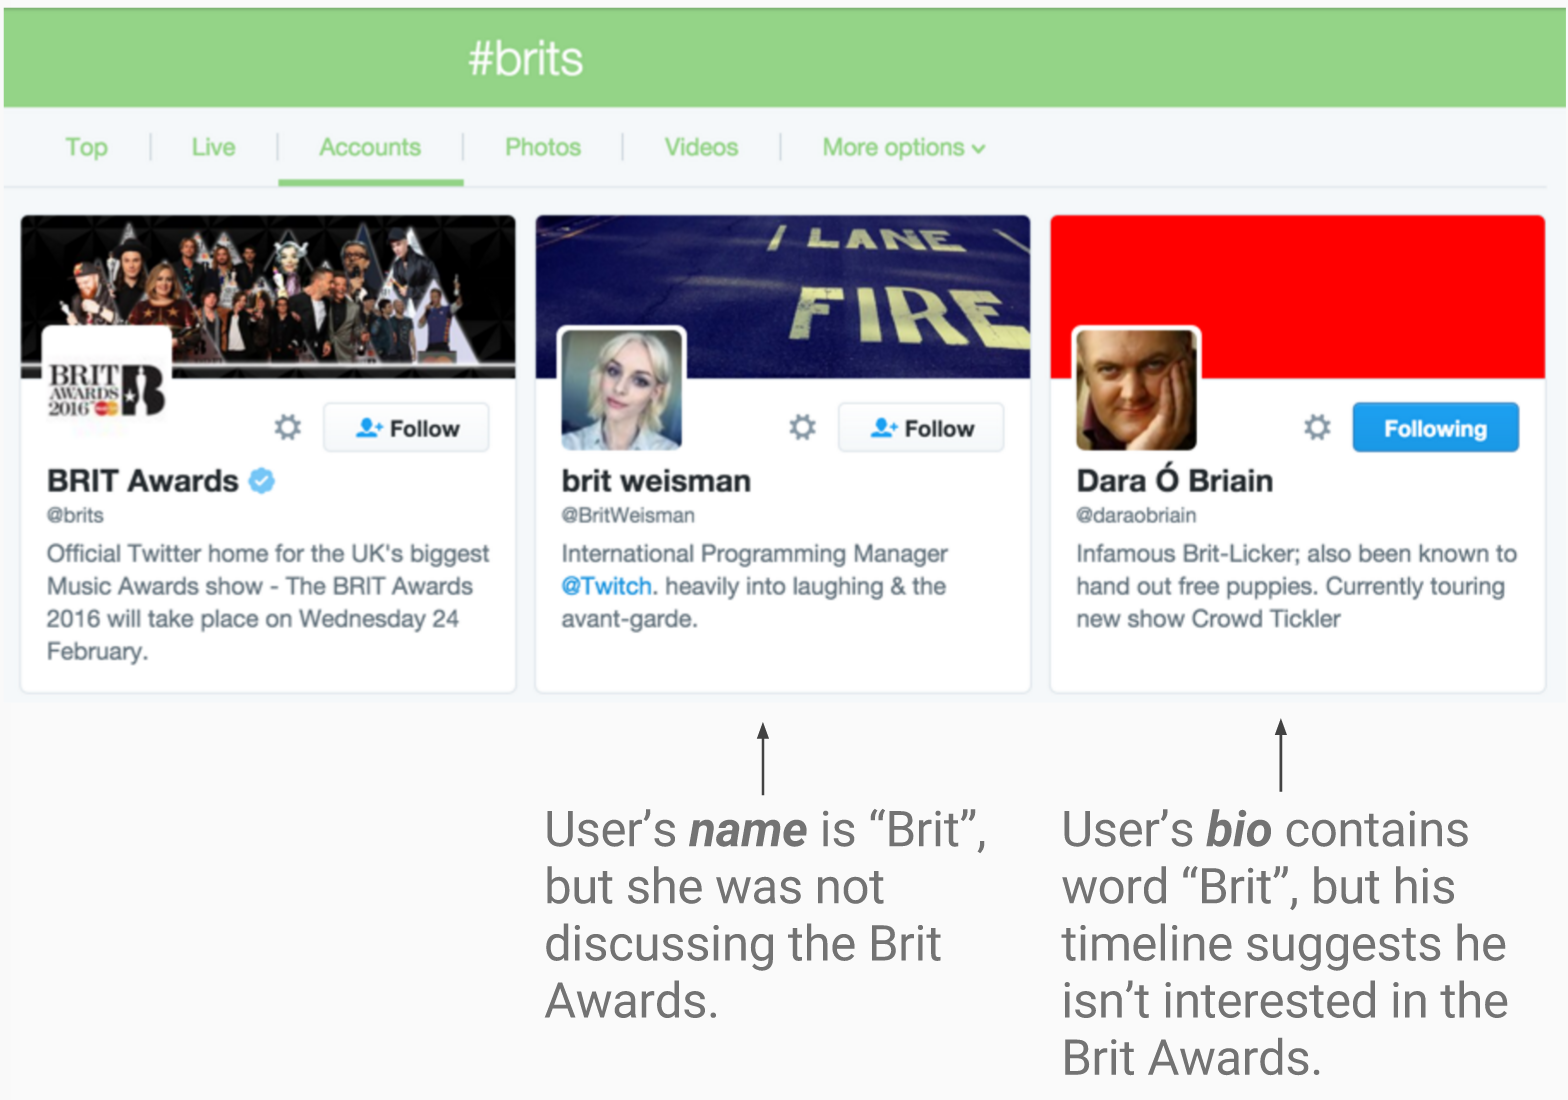
\includegraphics[scale=0.45]{twittersearch.png}
\caption{Twitter's own search service. Searching for a hashtag appears to either disregard or give very little weight to users who use the hashtag in their tweets.}
\label{twittersearch}
\end{figure}

In order to determine the short-term interests of Twitter accounts, the ``Who To Follow In Context'' project relies on the content of tweets recently posted by the account over their username and bio. Additionally,
evidence from new tweets is immediately applied, and suggestions update in real-time, modelling the evolving nature of the events that many users are interested in. If a query result page is left open, the ranking of accounts will be adjusted as people start and stop discussing the query topic, providing users with an insight into how new participants in the discussion emerge. This differs from Twitter Search, which provides a static set of results based on a query.

\subsection{Twitter's Whom To Follow Service}
``Whom To Follow'' (known as ``Who To Follow'' until March 2016) is the service used at Twitter which recommends accounts to follow based on the people already followed by an account. In order to do this, it relies on a ``user graph'' \cite{twitterWTF}. The user graph is a directed graph where vertices represent Twitter accounts, and edges represent a ``following'' relationship. That is, an edge $(A, B)$ in the directed graph means that user $A$ \textit{follows} user $B$ on Twitter, and is therefore subscribed to their tweets. 

\begin{figure}[H]
\centering

\includegraphics[scale=0.75]{whomtofollow.png}
\caption{The user interface of Twitter's Whom To Follow service}
\label{whomtofollow}
\end{figure}

Since the service relies on the relationships between users in the user graph, it suggests accounts similar to those that you already follow. While this provides excellent suggestions based on long-term interests, it cannot be configured or queried in order to provide recommendations under a different context (such as events). Additionally, recommendations for users are done in batches, and are therefore not updated in real-time. This means that even if the user graph did provide signals as to the immediate relevance of a Twitter user with respect to an ongoing event, it is likely that this relevance will have decayed by the time the recommendations are delivered.

Since the initial deployment of this service in 2010, Twitter announced they are reimplementing the service using Pig and Hadoop to improve scalability, and also to apply machine learning approaches using a wider variety of signals. It is unclear whether the new system is now in place.

\subsection{Klout}
Klout provides a well-known system for ranking the influence of users across numerous social media platforms and online communities. It takes into account over 3600 features from these sources, and processes around 500 million user interactions each day \cite{klout}. Although Klout does not attempt to solve the exact same problem as this project (Klout ranks users based on a static context: \textit{``How influential is this user?''} rather than their relevance based on a query), its well documented architecture and popularity in the domain make it worthy of mention.

\begin{figure}[H]
\centering
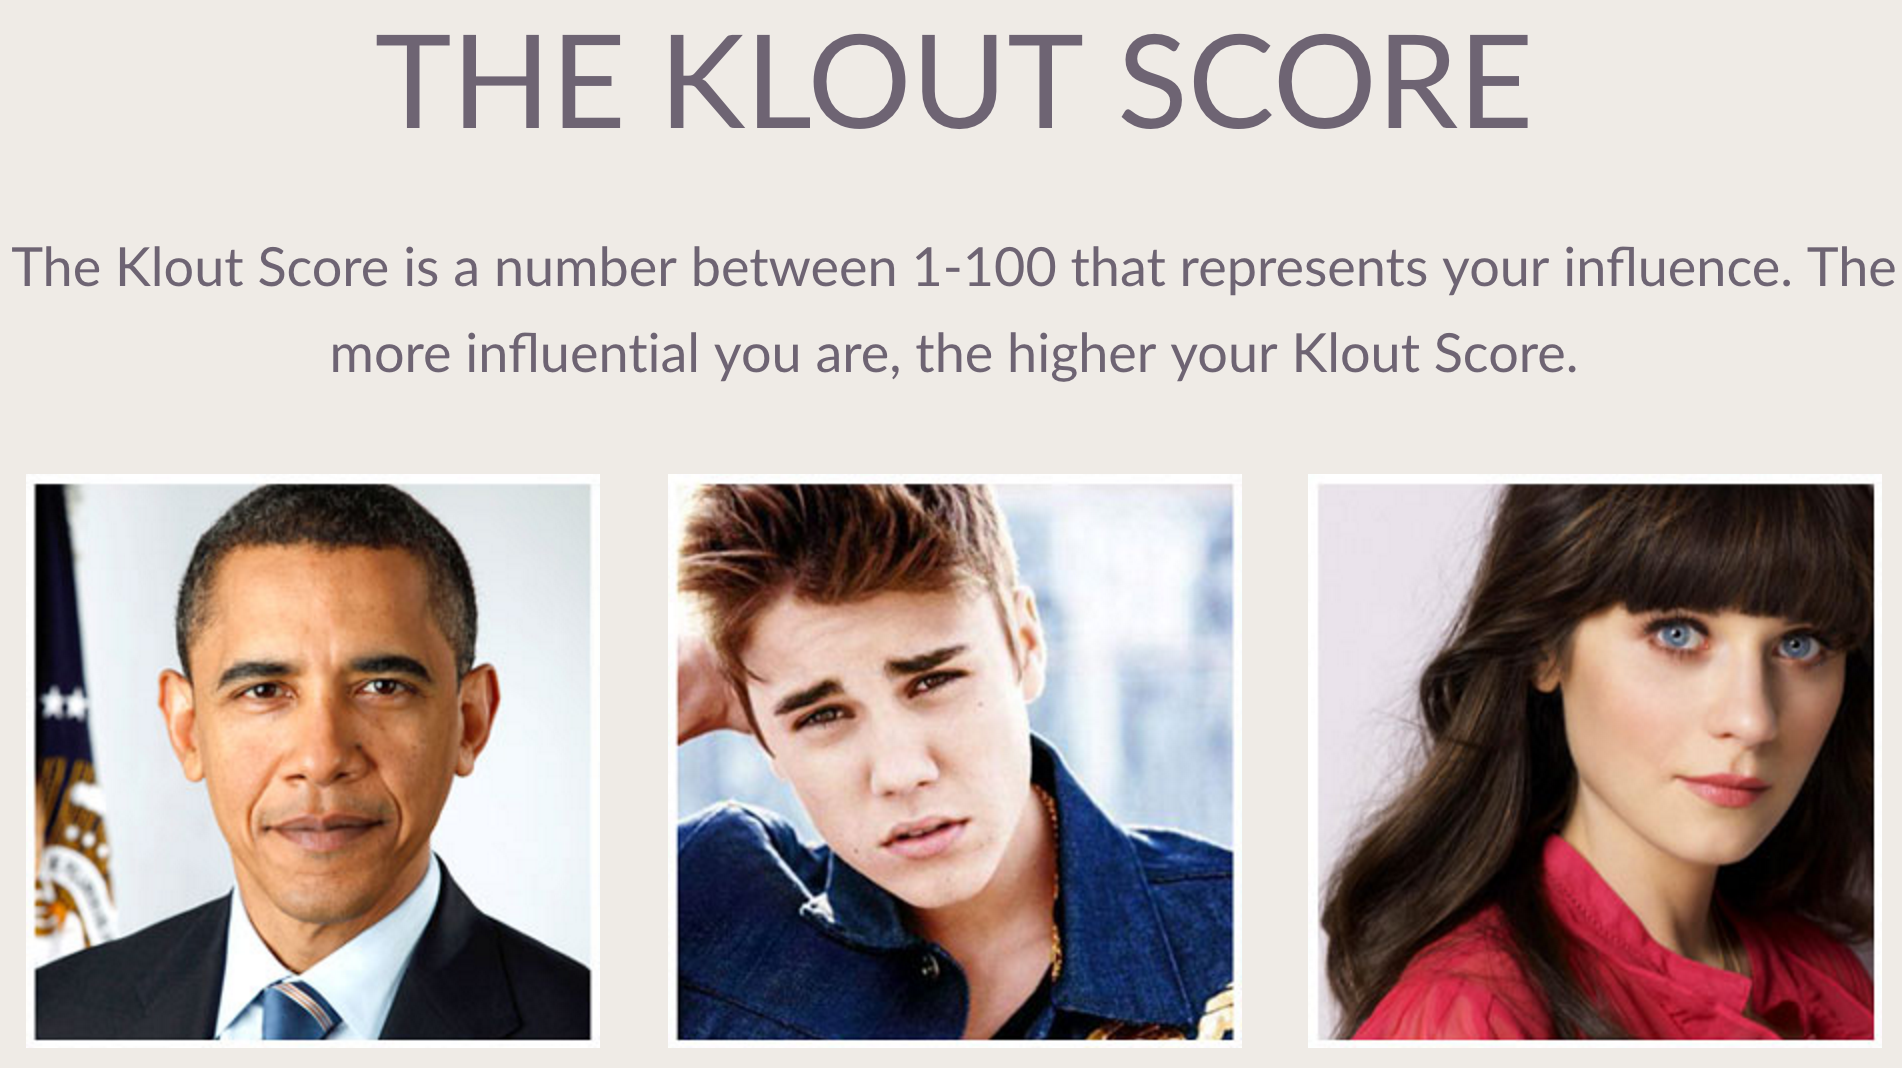
\includegraphics[scale=0.3]{klout.png}
\caption{The three users with the highest Klout scores.}
\label{kloutimage}
\end{figure}

\section{Relevant Research}

    \subsection{Searching For Quality Microblog Posts}
    This paper examines an array of metrics for examining whether a post on a microblog is high quality or not \cite{Vosecky2012}. It introduces an array of features which can be extracted from tweets, and examines the impact of the reputation of external URLs linked to from the tweet. Many of the techniques examined in this paper are applied in the filtering stages of this project, in order to discard tweets which do not meet a threshold on the extracted features.
    
\section{Summary}
After introducing the goals and motivations behind the project, existing services which tackle similar problems were examined. These services were shown to be effective at finding users based on their long-term interests, but to be lacking in the context of live events. The approach taken by the ``Who To Follow In Context'' application was also introduced, in terms of how it attempts to solve the flaws present in the existing services.

\chapter{Requirements}

Requirements were gathered during the initial meetings between the author and the project supervisor. These requirements were frequently updated as new considerations were made and new restrictions realised, but in general, they aimed to solve the issues that the related products listed in Chapter 1 have when it comes to live events. To ensure the customer (the project supervisor) that progress was being made in satisfying these requirements, weekly status reports were produced during the implementation stage. 

    \section{Functional Requirements}
    
    Functional requirements were gathered in order to describe the specific behaviours the system may offer. In order to prioritise these requirements, the \textit{MoSCoW framework} was used. That is, requirements were categorised in terms of their importance into the sets ``must have'', ``should have'', ``could have'', ``won't have''.
    
    \subsection{Must Have}
    
    Requirements listed in this section were vital to the success of the project. Without satisfying all of these requirements, the project would be regarded as unsuccessful. 
  
    The system \textit{must have} the following capabilities:
    \begin{enumerate}[label=\textbf{M.\arabic*}]
    \item Present a web-based user interface providing querying and result-viewing capabilities.
    \item Read tweets live from the Twitter Streaming API.
    \item Extract the following features from incoming tweets:
        \begin{enumerate}
        \item The length of the tweet.
        \item The number of correctly spelled words in the tweet.
        \item The number of capitalised words in the tweet.
        \item The hashtags used in the tweet.
        \item The number of ``likes'' the tweet had at the time it was processed. 
        \item The number of retweets the tweet had at the time it was processed.
        \item The number of URLs the tweet contains.
        \item The number of users mentioned in the tweet.
        \end{enumerate} 
    \item Filter out Twitter users who post low quality tweets.
   \item Index tweets and relevant metadata so that they can be quickly retrieved given a user query.
   
   \item Display the results of the query as they update in real-time.
   \item Display the timeline of Twitter accounts suggested by the application, without leaving the application. 
   \item Retrieve user suggestions based on an event identifying ``hashtag'' query.
    \end{enumerate}
    
        \subsection{Should Have}
        
        ``Should have'' requirements were considered important for the project, however they are not given the same level of importance as ``must have'' requirements. The exclusion of some of these requirements would not result in an unsuccessful project.
        
        The system \textit{should have} the following capabilities:
        
        \begin{enumerate}[label=\textbf{S.\arabic*}]
        \item Read historical tweets from a file to improve evaluation capabilities.
        \item When reading tweets from a file, any user timelines viewed should be a snapshot of their timeline corresponding to the time the tweets in the file were sampled from.
        \item Alter its behaviour according to options defined in a configuration file.
        \item Allow users to provide feedback in order to evaluate and improve the relevance of future results.
        \item Provide users with visual feedback to inform them of the current status of the system.
        \item Store tweet features and relevance judgements for evaluation purposes.
        \item Examine a user's timeline to for additional tweets that can be used as evidence for their relevance.
        \end{enumerate}

        \subsection{Could Have}
        ``Could have'' requirements are those that were not considered important, but could improve some aspect of the project such as result relevance or user experience.
        
        The system \textit{could have} the following capabilities:
        
        \begin{enumerate}[label=\textbf{C.\arabic*}]
        \item Show users any new queries as soon as they are entered in order to encourage interaction.
        \item The reputation of the URLs the tweet contains.
        \item The sentiment of the tweet (e.g. number of positive or negative emoticons used).
        \item Show how user relevance changes over time.
        \item Counts for several punctuation marks used within the tweet. Research has suggested that this may be an indicator of microblog post quality \cite{Vosecky2012}.
        \end{enumerate}
        
        \subsection{Won't Have}
        ``Won't have'' requirements are those which the student and project supervisor agreed should not be implemented.
        
        The system \textit{won't have} the following capabilities:
        \begin{enumerate}[label=\textbf{W.\arabic*}]
        \item Each query should result in a live stream of relevant tweets being displayed alongside the suggested results for that query. This feature was not implemented due to the restriction imposed by Twitter that each application can only have a single stream open.
        \item Provide the ability to ``follow'' users when providing relevance feedback
        \end{enumerate}



    \section{Non-Functional Requirements}
    
    In addition to the functional requirements defined in the previous section, as set of non-functional requirements were agreed on. These requirements describe criteria on how the system should be judged, rather than examining the behaviour it offers. The application was implemented and designed taking these requirements into account as much as possible.
    
    \begin{enumerate}[label=\textbf{N.\arabic*}]
    \item Support multiple users concurrently without there being a noticeable impact on performance.
    \item Support multiple queries concurrently without there being a noticeable impact on performance.
    \item Be robust enough to handle a variety of issues such as network problems without failing.
    \item Be constructed in a scalable manner so that it can easily be extended to run on a cluster of machines if required in the future.
    \item Be constructed in a maintainable manner.
    \item Display a response (whether that is results or an indication that no results were available) to queries within one second of them being issued.
    \item Operate within the restrictions imposed by the Twitter REST API v1.1 rate limits.

    \end{enumerate}

\section{Summary}
This chapter has presented both the functional and non-functional requirements for the ``Who To Follow In Context'' project. The functional requirements were prioritised using the MoSCoW framework, and this was used to steer the implementation of the project.

\chapter{Architecture}

This chapter describes the architecture of the system, and goes on to discuss how technologies used within this architecture were evaluated so as to best meet the requirements.
    
    \section{Model-View-Controller}
    The application loosely follows the \textit{Model-View-Controller} architectural pattern. This architecture consists of three high level layers: the \textit{model}, the \textit{view}, and the \textit{controller}. The model is responsible for the storage and retrieval of data based on instructions from the controller. The view is the user interface of the system, which users can interact with. These interactions are sent to the controller, which is the mediator of communication between the model and the view.
    
\begin{figure}[H]
\centering
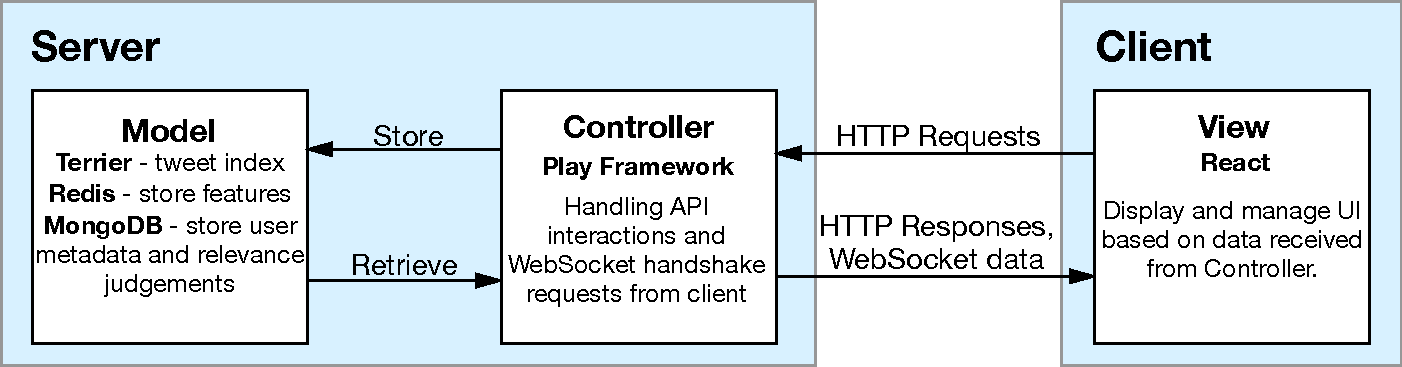
\includegraphics[scale=0.70]{mvc.pdf}
\caption{The high-level architecture of the application using the Model-View-Controller architectural pattern.}
\label{mvc}
\end{figure}

``Who To Follow In Context'' is designed with a web interface, as per requirement \textbf{M.1}. This interface is implemented entirely on the client, and communication between client and server is handled using HTTP (Hyper Text Transfer Protocol). The client can send HTTP requests to the server, and the controller will handle that request by communicating it to the relevant component within the application. HTTP requests sent from the view to the controller can either request that data be retrieved from or stored in the model layer. Additionally, an HTTP request can ask the server to upgrade the connection to a WebSocket \cite{websocket}. A request of this form is required in the case that a continuous stream of data is to be sent to the user (this is required to satisfy requirement \textbf{M.6}, for example).
    
    \subsection{Model Layer Technologies}
    Terrier, Redis, and MongoDB provide the persistence layer of the application. Each of these technologies provide different benefits and so the decision of which to use and where to use it varied depending on context.
    
        \subsubsection{Indexing Tweets}
        The model layer of the application contains an ``indexer'' component which stores incoming tweets in an index, so that they can be efficiently retrieved. The index structure used is provided by \textit{Terrier}, an information retrieval platform developed at the University of Glasgow \cite{macdonald2012puppy}. The \code{MemoryIndex} structure used enables the index to be built online, meaning that it can be queried as it is being constructed. This capability was vital in order to satisfy requirements \textbf{M.5} and \textbf{M.6}.
        
        \subsubsection{Feature Storage}
        \textit{Redis} is an in-memory data structure storage engine which is used for storage of extracted features (requirement \textbf{S.6})\cite{redis}. By keeping data in memory it enables quick reads and writes in comparison to on disk solutions such as relational or NoSQL databases. Therefore, at the cost of memory, the server spends less time reading and writing data and has more resources spare to perform other tasks. Redis's built in data structures also simplified the implementation of certain features. For example, a Redis SortedSet data structure is used for the calculation of the median time since the user last made use of the query term as a hashtag. Since the application must process vastly more reads than writes for individual users, allowing Redis to perform the sorting step at write time makes the system more efficient than if we were required to sort an array each time the latest results were retrieved for a user.
        
         \subsubsection{Miscellaneous Storage}
         \textit{MongoDB} is a NoSQL database used for the caching of Twitter user metadata in order to reduce the number of Twitter API requests required \cite{mongo}. This assists the application in staying within the restrictions of the Twitter API rate-limiting policy (as per requirement \textbf{N.7}). For example, we store the URL of the user's profile picture and timeline colour in MongoDB and check for its existence here before making an additonal API request for the information. We also store user relevance feedback in MongoDB for evaluation purposes.
         
         NoSQL was used due to the lack of need of relational features. Each category of item stored in this database is entirely independent from the others, and thus guaranteed that relational database features such as joins would not be necessary.

    \subsection{View Layer Technologies}
    
    The entirety of the ``view'' layer of the system is handled on the front-end. On receiving a request for the application's index page, the server will send an empty HTML document to the client containing only a ``mount'' element, which the client side will render the view within. The view layer is constructed using a number of different technologies such as TypeScript, React, and React Router.
    
    \subsubsection{Programming Language}
        The programming language used to create the front-end of the application was \textit{TypeScript}. TypeScript is a typed superset of JavaScript which provides compile-time type checking which eliminates a large number of run-time errors \cite{typescript}. Existing JavaScript libraries can be used from within TypeScript by including a ``type definitions'' file in the project. The purpose of such files is to provide a mapping from the non-typed JavaScript constructs to their corresponding TypeScript types. Since TypeScript is a type checked language, we also gain the benefits of code-completion and refactoring capabilities within certain integrated development environments.
        
        The front-end was initially written in JavaScript and then migrated to TypeScript as the number of type related errors began to increase due to the increasing complexity of the front-end. Although the initial migration to TypeScript was extremely time consuming, the number of run-time errors encountered significantly decreased, making the system far more robust than before (thereby furthering requirement \textbf{N.3}).
    
        \subsubsection{User Interface}
        The components which combine to form the overall user interface are written using \textit{React}. React is a JavaScript library developed by Facebook for constructing user interfaces in a component-based fashion \cite{react}. There is an abundance of modern libraries and frameworks for developing user interfaces. React was chosen primarily for its enforcement of the idea of ``separation of concerns'' and its renowned performance.
        
        The other popular client library considered for the project was AngularJS by Google \cite{angular}. However, Angular is framework rather than a library and as such forces the developer to write their application within its restrictions. Additionally, Angular is well known to have considerably worse performance in comparison to React, due to slower DOM (Document Object Model) manipulation operations \cite{reactvsangular}. Due to the fact that the view of this application updates frequently, performance of the view framework chosen was of paramount importance.
        
    The client side of the application is constructed as a single-page application (SPA) meaning that the entire application is mounted at a single URL (excluding API endpoints which return JSON rather than text/html content). Navigation between pages is then managed entirely by client-side code. The decision to make routing a concern of the front-end was driven by the existence of \textit{React Router} and the fact that the application view has a limited number of overall view states \cite{reactrouter}. Using this library allowed views to be declared hierarchically, so that only required subtrees of the view are re-rendered on a URL change.
Additionally, the entirety of the views are implemented on the client side, and data is fetched either via a REST API (as opposed to server-side rendering of views) or through an open WebSocket. This approach provides the benefit of reducing the number of requests made to the server, and greatly improves the responsiveness of the front-end. 

Although we gain an overall more responsive experience using this architecture, it does have some associated flaws. The initial page load is often slower, since the client contains more code than it otherwise would if rendering and routing was managed on the server. Additionally, the improvement in page load times can place a burden on the server, since it has to ensure that the data will be available when a user requests it. If the data is not available when required by the user, it may prove irritating as they wait on certain portions of the interface to update.

\subsection{Controller Layer Technologies}
        
        Since the product is implemented as a web application, the controller chosen must be able to mediate communication between client and server over HTTP.

        \subsubsection{Play Framework}
        The \textit{Play Framework} was used for its WebSocket implementation and to create REST API endpoints, such as the endpoint used in fetching the timeline and metadata for a user when they are clicked on in a result set \cite{play}. Since routing and rendering was done on the front-end, only a small subset of the features of Play were required. This framework provided the benefit of having excellent integration with other technologies used in the implementation, such as Akka (Play is also written using Akka) and Guice, allowing WebSocket connections to be accepted using actors. An additional benefit of using this framework is that it is one of the most popular web frameworks for Java and Scala, and as such it has an active developer community with clear and extensive documentation.
    
    \section{Server Architecture}
    Whilst interaction between the client and server follows the Model-View-Controller pattern, other components exist within the architecture which do not fit so precisely into this framework. These components perform a variety of functions, such as the processing of incoming tweets and the real-time reporting of system statistics. Figure \ref{architecture} shows how the system is designed in terms of the flow of data between components, and the following sections will describe the purpose and technology-related decisions behind each component.
    
\begin{figure}[H]
\centering
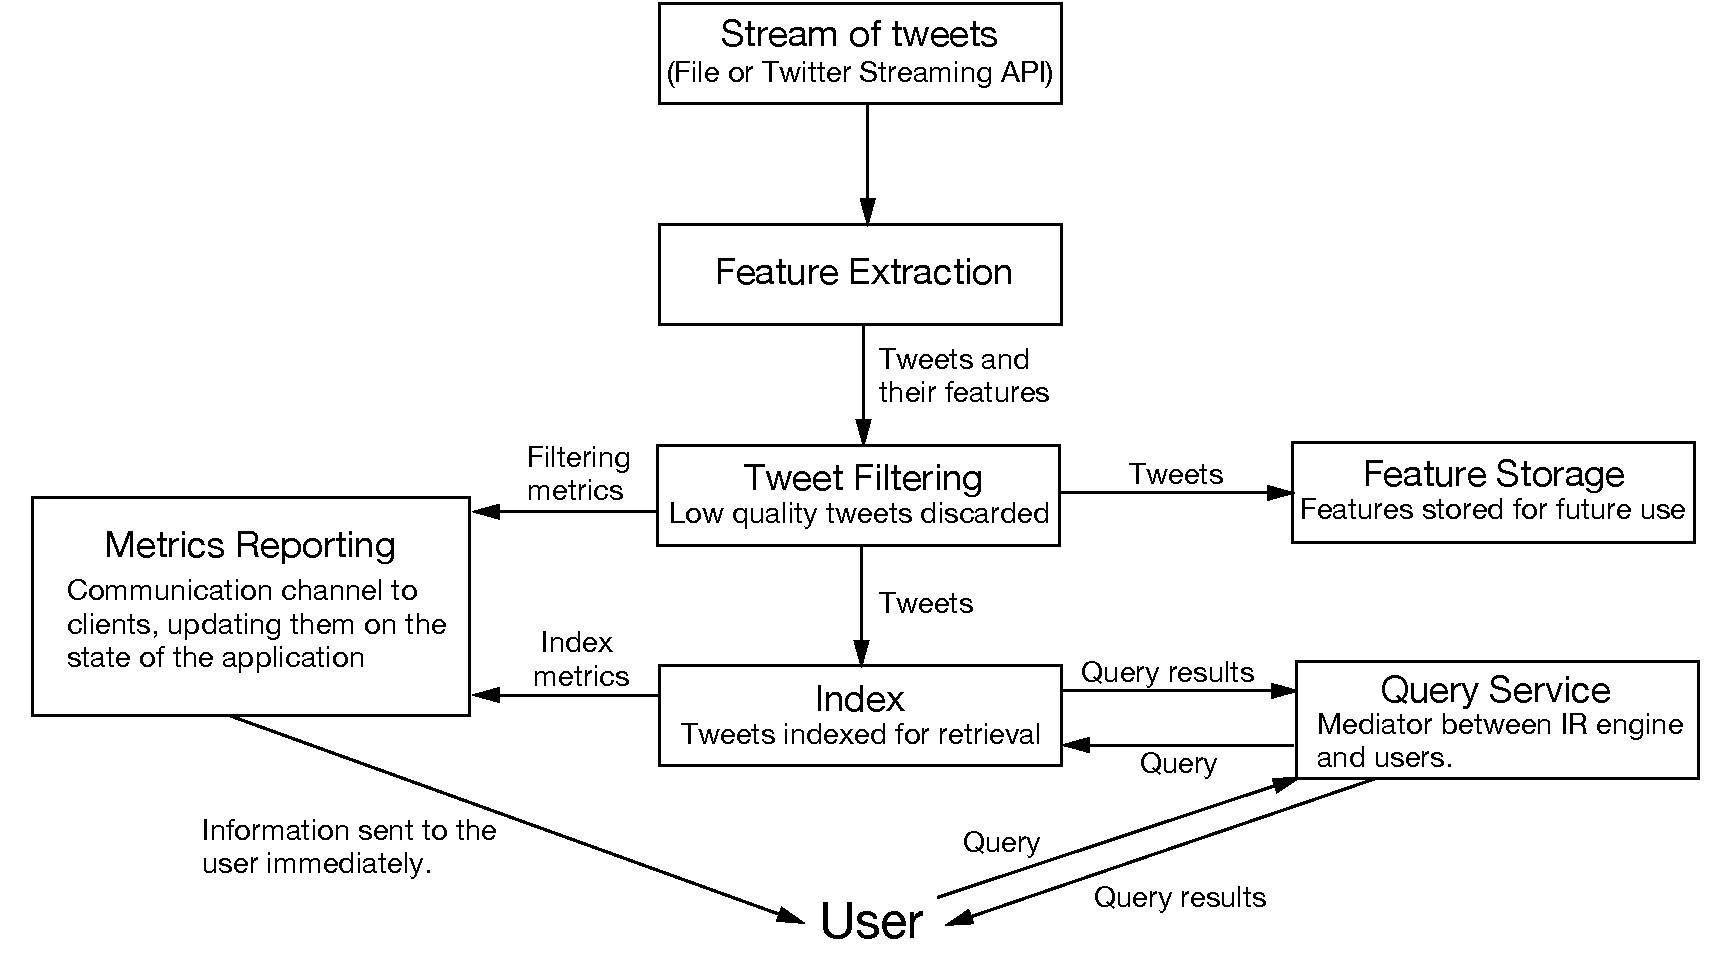
\includegraphics[height=278px,width=496px]{architecture.pdf}
\caption{The high-level view of the feature extraction pipeline of the system. The ``Implementation'' chapter looks at the internal workings of each component in detail.}
\label{architecture}
\end{figure}
    
    \subsection{Feature Extraction and Tweet Filtering}
        Incoming tweets are initially passed to the feature extraction component. \textit{Spark Streaming} (and Twitter4J for authentication purposes \cite{twitter4j}) provided a convenient way to access the Twitter streaming API, and distribute the feature extraction workload across multiple processing cores \cite{sparkstreaming}. Spark is designed to work in a distributed environment, and therefore also leaves open the possibility of distributing the stream across multiple machines in a cluster should the need arise. Spark was chosen over alternatives such as Apache Storm due to the fact that the author is more familiar with it, it has more extensive documentation, and it is known to work well with Akka (Spark is written on top of Akka), a technology used to maximise the concurrency within the application.
        
        The feature extraction component extracts features from the content of the tweet and its metadata, and thus (partially) satisfies requirement \textbf{M.3}. The intention of performing this extraction is to determine the quality of tweets. These features are passed to the filtering component which will discard tweets which do not meet a configurable quality threshold. The purpose of filtering these tweets is to prevent unnecessary computational load and also to avoid hitting the rate limiting restrictions of the Twitter API as per requirement \textbf{N.7}.
        
        After low quality tweets have been filtered (according to requirement \textbf{M.4}), the features of the remaining tweets are stored for future use, and the remaining tweets are progressed to the indexing stage of the pipeline.

Both the feature extraction and filtering components may receive tweets from other locations within the system. If the system ever deems a user to be relevant (for example, if they appear in a result stream for an open channel, or a user of the system views their profile), then the tweets present on that user's timeline are fed back into the pipeline in order to extract further evidence in the hopes of improving the relevance of results. This ability to examine a user's timeline is stated in requirement \textbf{S.1}.

        \subsection{Indexing \& Retrieval}
        After low quality tweets have been discarded, those remaining are sent to the indexer (part of the model layer) where they will be stored for efficient retrieval. 
        
        When a query is received, the Query Service will construct a result stream between the information retrieval engine and the user who entered the query. Terrier will then be frequently polled for new results, and the new results will be sent to the user as soon as they are available. Any user which enters the same query thereafter will see the same stream of results. The implementation details of this component are left for the ``Implementation'' chapter.
              
        \subsection{Metrics Reporting}
        Throughout different stages of the pipeline, different metrics are collected. These metrics are both logged and sent to the user in real-time to provide insight into the operation of the system (thus satisfying requirement \textbf{S.5}). This is important as it ensures the user that the system is working as expected. If a large period of time passes and no new users have appeared in the stream of results they are viewing, they might think that something has went wrong. By keeping them constantly updated on the number of users the application has processed, they are ensured that it is working as expected.
        
        Numerous different technologies were examined for providing this functionality, including the \textit{Comet model} in HTTP 1.X, the WebSocket protocol, and using the persistent connection and multiplexing capabilities of HTTP 2.0.
        
        Comet sockets were introduced to provide streaming capabilities before the introduction of the WebSocket API, and as such rely on many browser hacks to work properly \cite{comet}. However, with the correct hacks this provides excellent compatibility with older browsers which do not support WebSockets. Facebook Messenger is one such service that (as of 2013) relied on Comet for providing real-time notifications.
        
        HTTP 2.0 is the latest version of the HTTP specification which provides an abundance of new features and exceptional performance improvements over the currently dominant HTTP 1.X protocols \cite{http2}. These features (such as connection multiplexing) mean that the ``hacks'' required with the first version of the protocol which enable streaming are no longer required. However, support for HTTP 2.0 in existing libraries and frameworks are limited as of the time of writing. As such, relying on HTTP 2.0 would have added too much development overhead to make it practical.    
        
       After consideration of the above technologies, the WebSocket protocol was chosen to enable real-time communication between the server and connected clients \cite{websocket}. The WebSocket protocol is well supported in modern browsers, and is specifically designed for immediate, full-duplex (simultaneous, two-way) communication between client and server. Additionally, WebSockets are well supported in modern web frameworks meaning there is a large community of developers  and supporting documentation available.
          
        A downside of using a WebSocket reliant architecture is that the protocol is much slimmer than HTTP, and therefore it was required to implement the notion of a ``keep-alive'' to ensure that channels are cleaned up in the case that no client registers an interest in it.


    \section{Design Decisions}

    A number of decisions had to be made with regards to the overall architecture of the application. These included which programming language to employ, how to handle concurrency, and how to design the system so as to minimise the coupling between components.

    \subsection{Server Programming Language}
            The server is written using the statically typed \textit{Scala} programming language, which is a hybrid of the object-oriented and functional paradigms \cite{scala}. Scala was chosen for its lightweight syntax and the fact that it compiles to Java Virtual Machine byte-code, allowing for clean interoperability with existing Java libraries and frameworks. In fact, a number of extremely popular Java libraries are written in Scala, including Apache Spark, Akka, and the Play Framework. Additionally, Scala provides powerful means of asynchronous programming through \code{Future}s and \code{Promise}s, and its \code{Option[T]} type and powerful pattern-matching features make \code{NullPointerException}s impossible since it explicitly requires the developer to check for the possibility that the \code{Option[T]} type contains a \code{None} value. Scala also benefits from its powerful REPL (Read-Execute-Print Loop) which comes bundled with the Scala compiler. This allows developers to immediately evaluate expressions and see the results. Existing code can even be loaded into the REPL so that the effects of performing actions on user defined objects can be examined.
            
        Other languages examined in the initial investigations were Python \cite{python}, NodeJS \cite{node}, and Java \cite{java}. Python was ruled out due to its poor support for concurrency, and its dynamic typing would likely have caused difficulty as the complexity of the project source code increased. 
        
        NodeJS was considered for its renowned support for real-time web applications. However, the ecosystem surrounding the language has not expanded into the field of processing data streams. As with Python, NodeJS is dynamically typed, and this also factored into the decision to rule it out. 
        
        Finally, Java was considered due to its unmatched ecosystem of libraries and frameworks and its type system. Java has a massive range of libraries available, but they make excessive use of \code{null} values, which greatly increase the possibility of run-time failure. Java is also extremely verbose in comparison to Scala, as can be seen in Listings \ref{scala} (Scala) and \ref{java} (Java), which show Spark Streaming code for splitting a line from a text stream into an array of words.

\begin{lstlisting}[caption=Scala example of splitting a line in Spark Streaming.,label=scala]
// Split each line into words
val words = lines.flatMap(_.split(" "))
\end{lstlisting}

\begin{lstlisting}[language=Java,caption=Java example of splitting a line in Spark Streaming,label=java]
// Split each line into words
JavaDStream<String> words = lines.flatMap(
  new FlatMapFunction<String, String>() {
    @Override public Iterable<String> call(String x) {
      return Arrays.asList(x.split(" "));
    }
  });
\end{lstlisting}




    \subsection{Concurrency Model}
    
    The real-time nature of the application means that if response times are poor then it will immediately impact user experience. Should feature extraction for a batch of tweets from a user's timeline take longer than expected, then a user will have to wait until the system gets around to processing that user. As such, high levels of concurrency were deemed vital in order to meet user requests in a timely manner (as stated in requirements \textbf{N.1} and \textbf{N.2}). To accommodate such a requirement, the system was designed using the \textit{Actor model}.
    
    \subsubsection{The Actor Model}

Actor systems provide an alternative means of concurrency that avoid the pitfalls of typical synchronisation methods such as the use of shared mutable state and locks \cite{actormodel}. The actor model of concurrency was first popularised by the Erlang programming language, and has increased in popularity in recent years with the release of applications such as WhatsApp which use the model extensively \cite{erlang}. An actor system consists of a set of actors. Actors are entities capable of performing some computation on a thread in response to messages. Actors also have the ability to create new “child” actors, and to send messages to other actors in the system, who will then react in their own way depending on the information contained within that message. By communicating between actors solely through asynchronous \textit{immutable} message passing, we guarantee that the computations performed by a single actor cannot result in issues such as thread interference.

\subsubsection{Akka}

    \textit{Akka} is a framework for Scala and Java which implements the actor model \cite{akka}. Despite vastly simplifying the concurrency aspect of the implementation, Akka required very little overhead in terms of memory. The actor model framework provided by Akka supports passing approximately 50 million messages per second on an average machine, and around 2.5 million actors can exist per gigabyte of heap space. Each component of the architecture was implemented as one or more actors, and communication between components in the system was facilitated through message passing.
                    
        Despite being primarily used for its concurrency model, Akka provided a number of features ``out-of-the-box'' which satisfied several project requirements. Actors in Akka have a ``supervision strategy'' which defines what actions should be taken when an exception occurs within them. This allows the system to meet the high degrees of fault tolerance and resilience required. The default supervision strategy (simply restarting the actor when an exception occurs) solved many issues that were encountered. For example, it was common for the Twitter streaming API to become unavailable (due to network issues) and an exception was therefore thrown. The actor handling the stream was automatically restarted and the stream handle resent to all of the actors that required access to it. No explicit error handling code was required, yet the application was able to self-heal and become fully functional as soon as the streaming API became available again. As a result, using Akka greatly assisted in furthering requirement \textbf{N.3}.

        \subsection{Reactive Systems}
        The architecture of the system is implemented to conform to many of the tenets described in the ``Reactive Manifesto'' \cite{reactive}. That is, the system architecture is designed to be responsive, resilient, elastic, and message-driven. It was hoped that this architecture would assist in the satisfaction of several of the non-functional requirements listed in the previous chapter.
        
            \subsubsection{Responsiveness}
            Responsiveness is a key aim of the design. Messages passed between actors in potential areas of bottleneck are load-balanced in order to minimise the work queued on a single actor or thread and maximise throughput. Within each defined actor is a response time guarantee which, if not met, causes the actor to be restarted in attempt to regain responsiveness. 
            
            \subsubsection{Resilience}
            The application provides the guarantee of resilience through ``self-healing''. Should an actor executing some computation encounter an exception, its parent is notified and takes the appropriate action in order to cleanly recover. Additionally, if an exception occurs within any actor, it is treated in isolation, and other actors are not affected unless the parent actor's supervision strategy explicitly calls for it. Therefore, problems are compartmentalised and the cascading effect of errors spreading through the system is reduced.
            
            \subsubsection{Elasticity}
            Some actors within the system are implemented as state machines with the ability to change their behaviour at run-time, in response to certain events. This can be useful, for example, if the application hits the Twitter API rate-limit. The behaviour of the corresponding actor can be modified to stop making API requests for a specified period of time, and then modified back to its original API-reliant behaviour after this time period has expired.
            
            \subsubsection{Message-Driven}
            The architecture is entirely message driven. The root messages are batches of tweets read from a stream of tweets, or user interactions with the system. Each of these messages results in a chain of messages being sent asynchronously between actors as they handle the situation. Using a message driven architecture also provides an excellent abstraction for handling real-time data processing.      
        
        \subsection{Dependency Injection}
        
        The system relies heavily on the \textit{dependency injection} design pattern. This pattern greatly reduces coupling between components, and enforces a separation of concerns by separating dependency creation from behavioural code \cite{di}. By making extensive use of this pattern, requirement \textbf{N.5} is further satisfied.
        
            \subsubsection{Google Guice}
                
        \textit{Google Guice} is a dependency injection framework for Java which manages the dependency graph that exists between objects in an object-oriented environment \cite{guice}. Using Guice, one can request an instance of an object when required by ``injecting'' the instance into a ``setter'' method or a constructor.

Guice was primarily used for the injection of actor references into other actors. If we ever wish to send a message to an existing actor in order for it to perform some computation, we simply ask Guice for the instance of the required actor by injecting the actor into the constructor of the current class using the \code{@Inject} and \code{@Named} annotations provided by the framework.

    \section{Summary}
    The architecture of the system uses a number of different technologies which were chosen because it was believed that they would make improve the implementation of the project in some way. The technologies chosen for both client and server emphasise were picked so as to maximise the use of good software engineering principals.
        

\chapter{Implementation}
                    
Both client and server side were implemented so as to resemble the architecture described in the previous section. This chapter will examine the implementation challenges that arose during the construction of both client and server.

\section{Server Implementation}

    The server was implemented using many software development tools and practices. It consists of a number of different components, as was displayed in Figure \ref{architecture}. This section aims to examine several of these components in greater detail by looking at some of the considerations and challenges that were had during their construction.

    \subsection{Tools \& Practices}
    The implementation of the server involved a wide range of tools and practices which aimed to assist in the development process. These tools ranged in purpose from simplifying source code management, to building and executing the application.
    
             \subsubsection{Git \& Continuous Integration}
         \textit{Git} is a distributed version control system which was used extensively during the development of the project \cite{git}. A working implementation of the project was always maintained on the \code{master} branch. Features were developed on their own branches so as to not interfere with \code{master}. These branches were frequently merged into the \code{master} branch so as to avoid ``integration hell'', whereby feature branches become so complex that it is extremely difficult to resolve conflicts when merging.
         
             \subsubsection{GitHub}
             The project repository is also linked to a remote repository hosted on \textit{GitHub} \cite{github}. By hosting on a remote repository, we avoid the consequences of local disk failure, since there will always exist a recent backup of the project. Hosting a remote repository is also beneficial in that it makes the project more portable, since it can be cloned onto another machine.
             
             \subsubsection{Agile Software Development}
             The \textit{Agile} software development process was followed throughout the lifetime of the project. Although there was an initial requirements gathering stage, these requirements frequently changed, and the product itself changed as a result. The project was implemented with the knowledge that requirements are highly dynamic, and no commitment was ever made to any single implementation.
             
             \subsubsection{Kanban \& Trello}
             Project task management was done using the ``Kanban'' system \cite{kanban}, where projects are represented as a set of named lists and cards. \textit{Trello} is an online platform which implements this system, and it was used extensively throughout all stages of the project \cite{trello}.
         
             \subsubsection{SBT (Scala Build Tool)}
         \textit{SBT} is a build management system commonly used in Scala projects \cite{sbt} which is similar to popular Java build tools such as Maven \cite{maven}. SBT was used in the project to maintain and resolve dependencies, run tests, and to build and run the project.

    
% Each subsection should be modelled around one of the components mentioned in the requirements section. 
    
    \subsection{Feature Extraction}
        
        As described in the chapter on ``Architecture'', and shown in Figure \ref{architecture}, the feature extraction component extracts several features from incoming tweets. These features aim to classify the tweet as either high-quality or low-quality. In order to implement this component, Spark Streaming was used to distribute computation across multiple threads.
        
        Spark Streaming provides us with a \code{ReceiverInputDStream[Status]} (discretised stream) representing the incoming stream of tweets. The tweet stream was mapped to a ``windowed'' tweet stream. This allows us to view the stream through a ``sliding window'', and perform operations on these individual windows of tweets. The tweets in each window are batched and sent through the rest of the pipeline together. The width of the sliding window is defined temporally, as is shown in Figure \ref{slidingwindow}.
        
\begin{figure}
\centering
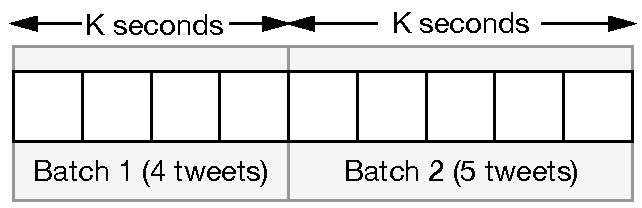
\includegraphics[scale=0.8]{slidingwindow.pdf}
\caption{Tweets are batched temporally and sent throughout feature extraction together.}
\label{slidingwindow}
\end{figure}

        The \code{FeatureExtraction} actor maps our windowed stream of tweets into a windowed stream of tweet feature vectors, which is immediately filtered to discard those tweets which do not meet the threshold quality criteria. These features are then sent to Redis for storage, and the original status is sent to the indexing actor for storage in a Terrier \code{MemoryIndex}.
        
        In early iterations of the project, features were stored in MongoDB \cite{mongo}. However, this proved to be a bottleneck on performance, since the implementation was unable to keep up with the rate at which new features were extracted. There are several reasons which explain why this situation occurred:
        
        \begin{itemize}
        \item MongoDB persists data on disk, resulting in slow read/write times compared to in-memory solutions.
        \item An asynchronous MongoDB driver was not used and so blocking occurred frequently.
        \item MongoDB does not have built-in data structures that could be used to avoid additional computations.
        \item Parallel insertions were not used. The MongoDB Scala driver had no serialisation/deserialisation support and this made using the parallel insertion API overly cumbersome.
        \end{itemize}
        
        To overcome this bottleneck Redis \cite{redis} was employed as the storage engine for features. This resulted in immediate performance improvements, but the system was still unable to store features at the rate they were being generated. Three additional steps were taken in order to ensure that features were persisted at an acceptable rate:
        
        \begin{itemize}
        \item Connection pooling was used to ensure that the application did not have to reconnect to the Redis server with each request.
        \item Requests to read and write features from Redis were partitioned by defining a \code{RedisRequest} type with two subtypes: \code{RedisReadRequest} and \code{RedisWriteRequest}. This allowed for the separation of reads and writes so that they can be processed by separate worker pools.
        \item Read and write requests were sent to a ``routing'' actor (named \code{RedisActor}) which maintains two pools of actors: one pool containing workers which deal with reading and unmarshalling data from Redis, and one containing workers which handle storing new features to Redis. These requests are distributed to workers using a Round-Robin algorithm, to ensure that the work is evenly distributed. Figure \ref{loadbalancing} shows how tasks were distributed between workers to maximise concurrency.
        \end{itemize}


\begin{figure}
\centering
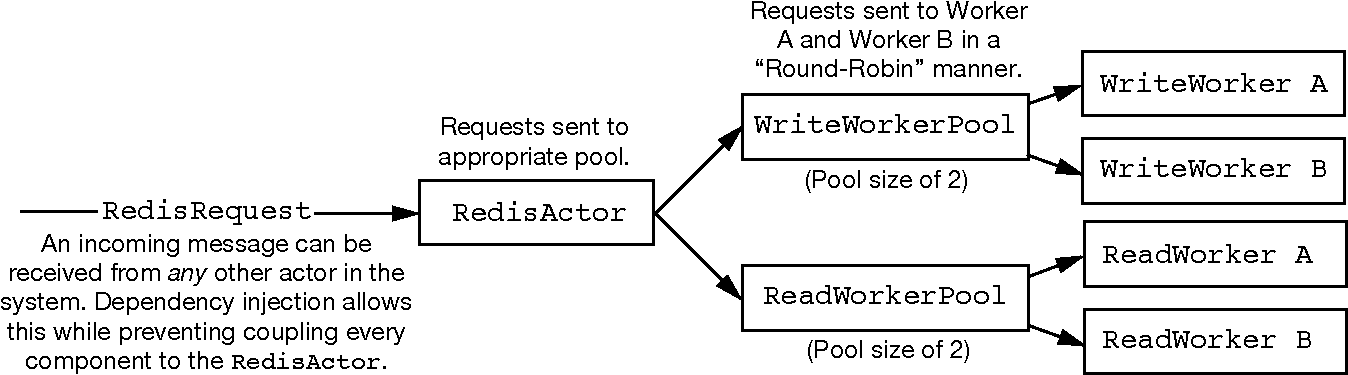
\includegraphics[scale=0.7]{loadbalancing.pdf}
\caption{An example of how requests were load-balanced in order to prevent overworked actors and maximise concurrency. This is a lower level view into the inner workings of the ``Feature Storage'' component shown in Figure \ref{architecture}}
\label{loadbalancing}
\end{figure}
        
        Akka made implementation of this load balancing simple since it provides extensive built-in support for such tasks, including protocols much more advanced than the Round-Robin method used in this component. The code for implementing a worker pool was a single line, as can be seen in the code for creating the \code{WriteWorkerPool} shown in Listing \ref{actorpool}.
        
        \begin{lstlisting}[caption=Creating an actor pool to reduce the work required by any single actor.,label=actorpool]
          val writingWorkerPool = context.actorOf(RoundRobinPool(4)
                .props(Props[RedisWriterWorker]), "writingWorkerPool")
        \end{lstlisting}

        
        After implementing the feature storage component using these techniques, it was found that it no longer restricted overall system performance.
        
        \subsection{Batched Feature Extraction}
        When a user becomes relevant and is displayed on an open result stream, their latest tweets are fetched (unless their timeline has already been processed recently). As a result, the number of tweets that we must process increases. If $N$ users become relevant at once, we will typically have around $20N$ additional tweets to process  (since we process the 20 most recent tweets from a timeline) on top of the tweets being processed from the stream. It is important in this case that there is no serious impact on performance.
        
        To minimise the disruption caused by any sudden influx of new tweets, extraction of features from tweets from a user's timeline was performed using the \code{Future} asynchronous programming abstraction provided by Scala. A \code{Future} represents a value that may become available \textit{at some point in the future}. Therefore, the value contained within a \code{Future} cannot be used until an associated computation is completed. A \textit{callback function} can be used to access the value when it is available.
        
        Since we want to avoid extracting features for the same tweet twice, we must check to see if the tweet has already been processed. To do this, we \textit{ask} the \code{RedisActor} if this is the case by sending it a message asynchronously. This actor has to go and do additional work to figure out how to reply, and therefore will not be able to respond immediately. Since the response is delayed, a \code{Future} is an ideal abstraction. The annotated code in Listing \ref{asyncfutures} shows how for each status in the batch we check if it has been processed in a non-blocking way. (Note: the \code{?} syntax is how we asynchronously send another actor a message and capture the eventual response in a \code{Future}.)
        
\begin{lstlisting}[caption=Check asynchronously whether a status has already been processed.,label=asyncfutures]
var tweetAnalysisHistory = 
    scala.collection.immutable.Set.empty[Future[(Long, Boolean)]]
// No iteration of this loop blocks waiting for a response, ensuring that
// every ask is sent immediately rather than after the response of the 
// previous ask
tweets.foreach(tweet => {
    // Add the Future representing the redisActor's eventual response to the set
    tweetAnalysisHistory += 
        (redisActor ? HasStatusBeenProcessed(tweet)).mapTo[(Long, Boolean)]
})
\end{lstlisting}
        
\code{tweetAnalysisHistory} is a set of \code{Future}s, each of which will eventually contain a pair of the form (TweetID, Boolean), where the boolean value is true if the tweet already been processed. Only after \textit{all} of these \code{Future}s are complete can we determine which tweets we have seen before and so will be discarded.

To determine when all of the \code{Future}s in the set are complete, we can \textit{compose} them into a single combined \code{Future}. Specifically, the set of type \code{Set[Future[(Long, Boolean)]]} is mapped to the type \code{Future[Set[(Long, Boolean)]]} using the \code{Future.sequence} method. Thus, rather than writing a callback function for every status in the set (which itself is impossible since we cannot know its cardinality until run-time), we can write a single callback function to handle the case where all \code{Future}s are complete, and this gives us access to the \code{Set[(Long, Boolean)]} contained within. The code showing this process is shown in Listing \ref{composefutures}, and has been annotated with comments and types for clarity (adapted from  \code{BatchFeatureExtraction.scala}).

\begin{lstlisting}[caption=Composing Futures unto a single future and registering the onComplete callback.,label=composefutures]
// Compose the Futures in tweetAnalysisHistory and register the
// callback to be fired when the composed Future completes.
Future.sequence(tweetAnalysisHistory) onComplete {
    case Success(seenBefore: Set[(Long, Boolean)]) =>
        // Future completed successfully, perform feature extraction
        // Original tweet list is filtered and feature extraction occurs here.
        ...
    case Failure(error) =>
        // Future unsuccessful, an actor may have missed response time guarantee
        // Error is logged
}
\end{lstlisting}

The feature extraction code itself (contained in the ``Success'' case of the pattern matching expression in the snippet above) is computationally expensive and as a result also relies heavily on asynchronous constructs, and uses many of the techniques described in this section.

        \subsection{Indexing}
        Tweets received at the indexing component are stored in a Terrier \code{MemoryIndex}. This is a special type of index that can be updated  online, and therefore is especially suited to this application. Each document stored in the index consists of one or more tweets from a single Twitter user. More specifically, the index stores a mapping from the terms in tweets to lists of Twitter users who have used that term. By storing data in this way, Terrier can achieve an $O(1)$ lookup of every user who has used a query term, allowing it to carry out retrieval quickly and efficiently. Since the index is stored in memory, further work will be required to ensure that the index is at least partially stored on disk when memory usage becomes too high.
        
        A secondary, ``metadata'' index is also maintained. The purpose of this index is to quickly retrieve metadata for any users it retrieves. Terrier will fetch only the document ID (equivalent to the Twitter user ID) for relevant users, and this auxiliary structure allows us to retrieve the metadata associated with that ID. The benefit of doing this is that it avoids the need to ask the Twitter API for that information just to display the results to the user. Preventing overuse of the Twitter API was a key aim of the application, as stated in non-functional requirement \textbf{N.7}. The metadata stored in this structure for each user includes their username, their screen name, and their profile biography.
        
        \subsection{Retrieval}

        To maximise performance, it was important to ensure that two users entering the same query does not result in the system computing the same stream of results twice. The traditional means of preventing this is through caching query results. Unfortunately, caching is not as practical in a system that is performing real-time indexing and providing results as a stream, since the results of a query change so frequently.
        
        To get around this limitation, each new query received opens a ``channel'', which the results of that query are forwarded through. The results that get forwarded through the channel are constructed by repeated polling of Terrier. Since the index is being constructed online, these results will be modified as the contents of the index changes. Every change in the set of results that is returned is sent through the channel to any connected clients. Clients can then use this data to re-render the user interface to display these changes. Figure \ref{channels} gives a simplified example of what the clients/channels relationship may look when the system is running. When a user inputs a query to the system, they are connected to a channel and will see the same stream of results for that query as any other user who has entered the query. If the channel corresponding to their query does not already exist, then it is created.
        
\begin{figure}
\centering
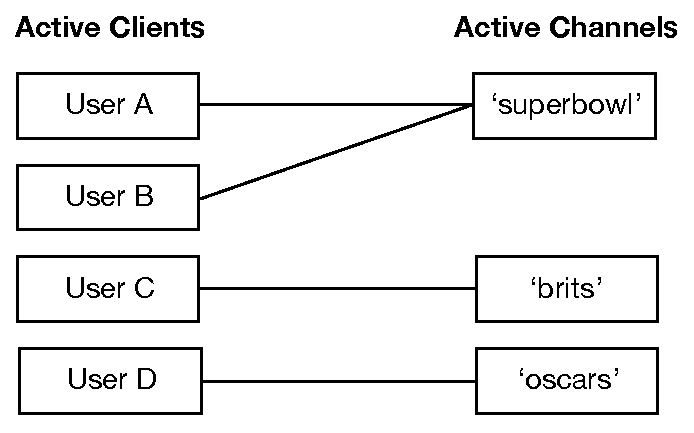
\includegraphics[scale=0.75]{channels.pdf}
\caption{\textit{An example of the one-to-many relationship that exists between users and channels}. Users A and B both connect to a single channel after entering the same query (``superbowl''), and will receive the results it outputs. This channel will perform the exact same actions regardless of the number of users connected.}
\label{channels}
\end{figure}     
        
        When a channel is created, it registers a scheduled request to poll Terrier for the latest result set in a configurable interval. The code in Listing \ref{pollterrier} shows how the polling rate was read from a dependency injected configuration file in a way that avoids \code{null} values, and then used to schedule the channel's work.
        
        \begin{lstlisting}[caption=Reading configuration from a file and scheduling the updates of results.,label=pollterrier]
          // Read the polling duration from the config file  
          val resultPollDuration = config.getInt("results.pollingrate").getOrElse(1000)
          
          // Schedule the requests for the latest query results
          val fetchTick = context.system.scheduler
                .schedule(Duration.Zero, FiniteDuration(resultPollDuration, TimeUnit.MILLISECONDS), self, FetchLatestQueryResults)
        \end{lstlisting}

        Through repeated polling, the result sets obtained from Terrier were transformed into a stream of results and sent to clients. These result sets are calculated using the BM25 weighting model, which is a popular information retrieval model known to generally give relevant results across a variety of test collections. Further investigation would be required to determine the most effective retrieval technique.
        
        Channels will remain open for a query for as long as at least one user is connected to the result stream. In order to determine whether any user is interested in the channel, connected users automatically send special ``keep-alive'' messages that the server interprets as a user expressing a desire to keep the channel open. Each open channel monitors the timestamp associated with the latest keep-alive received, and will free its associated resources if the latest keep-alive is ever older than some configurable threshold. In this way we ensure that a channel is never closed while a user is viewing a stream of results. Using this technique also allows us to close result streams when they are no longer required and therefore prevents resource leaks.
        
     
        
    \subsection{Metrics Reporting}
    This component is implemented as a single actor which can receive data from any other component in the system. By sending information to this actor, and specifying how it should translate this information (e.g. a Scala case class) to JSON, it allows any component to communicate with the client. In the example shown in Listing \ref{forward}, the \code{MetricsReporting} actor receives a message from some other actor informing it of the number of Twitter users that have been processed, and sends this message to all connected clients.
    
    \begin{lstlisting}[caption=Forwarding new messages through the WebSocket to connected clients.,label=forward]
      override def receive = {
        case numUsers @ NumberOfUsersSeen(_) => 
            channelMeta.channel push Json.toJson(numUsers)
        ...
      }
    \end{lstlisting}

The code which maps user-defined Scala types to valid JSON relies on the Play Framework's ``Writes'' converters. The converter for the example above is shown in Listing \ref{writesconverter}.

    \begin{lstlisting}[caption=Code for conversion of the NumberOfUsersSeen Scala case class to JSON format.,label=writesconverter]
      implicit val numberOfUsersSeenWrites = new Writes[NumberOfUsersSeen] {
        def writes(numberOfUsersSeen: NumberOfUsersSeen) = Json.obj(
            "numUsersSeen" -> numberOfUsersSeen.numUsers
        )
      }
    \end{lstlisting}

\subsection{Real-time Trending Hashtags}

One of the more interesting features to implement was the real-time hashtag usage counter. This component counts the number of occurrences of each hashtag within a configurable window of time, and updates this number as more tweets are processed. The user interface of this aspect of the system is shown in Figure \ref{trending}. The code which generates the data for this component is written using Apache Spark Streaming, and consists of several steps which in combination produce an output of \code{(hashtag, count)} pairs which are then sent to connected clients for rendering.

The initial step of this process maps the incoming stream of tweets into a stream of \code{(String, Int)} tuples, where the string is the text of the hashtag and the integer is the value 1. Figure \ref{mappingstep} shows this process diagrammatically, and the code used in this mapping process is shown in Listing \ref{tweetstohashtags}.

\begin{lstlisting}[caption=Initial mapping of tweets to hashtags pairs.,label=tweetstohashtags]
    // Map the tweets in the stream to a stream of (hashtag, 1) tuples
    val hashtags = stream flatMap(status => {
      status.getHashtagEntities map(hashtag => (hashtag.getText toLowerCase, 1))
    })
\end{lstlisting}

\begin{figure}
\centering
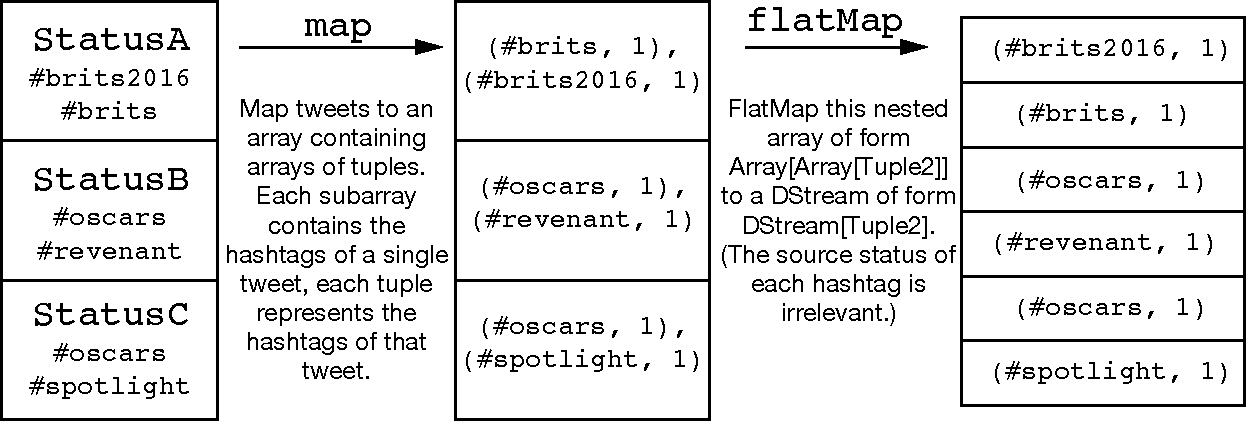
\includegraphics[scale=0.75]{mappingstep.pdf}
\caption{Example of how a tweet stream is mapped to a stream of pairs in the initial step of the real-time hashtag counting process.}
\label{mappingstep}
\end{figure}
               
The new stream of tuples is then \textit{reduced} within a sliding window using the \code{reduceByKeyAndWindow} operation provided by Spark Streaming. This operation takes place based on the key of the tuple (the first element; in this case the hashtag), and is analogous to a ``\code{GROUP BY}'' clause in SQL combined with a custom \textit{reducer function} which tells Spark how to reduce/combine two values from the stream into one. Since the stream is an array of tuples of the form \code{(<hashtag>, 1)}, after grouping by the hashtags, we want to reduce these tuples by summing their values in order to count the total number of times the hashtag has occurred in the stream (within the current window). Therefore, our reducer function is a simple addition:

\begin{lstlisting}
(p: Int, q: Int) => p + q
\end{lstlisting}

After applying this reduction, the data in the stream is now of the required form. After sorting the stream, a subset of the results are sent to the client to be displayed to connected users. The code which performs windowed reduction, sorts the results, and sends those results to all connected clients is shown in Listing \ref{reduce}.

\begin{lstlisting}[caption=Counting the hashtags used within a temporal window.,label=reduce]
    // Aggregate hashtags within the window
    val hashtagCountInWindow = hashtags
      .reduceByKeyAndWindow(
        (p:Int, q:Int) => p+q, Minutes(trendingHistoryMins), Seconds(reportFrequency)
      )
      .map{case (hashtag, count) => (count, hashtag)}  // Reverse tuples
      .transform(_.sortByKey(ascending = false))  // Sort by counts
      .map{case (count, hashtag) => HashtagCount(hashtag, count)}

    // Send latest trending data to connected clients
    hashtagCountInWindow foreachRDD(rdd => {
      val hashtagCounts = rdd.collect take numberOfHashtagsToShow
      metricsReporting ! TrendingHashtags(hashtagCounts.toList)
    })

\end{lstlisting}

\begin{figure}
\centering
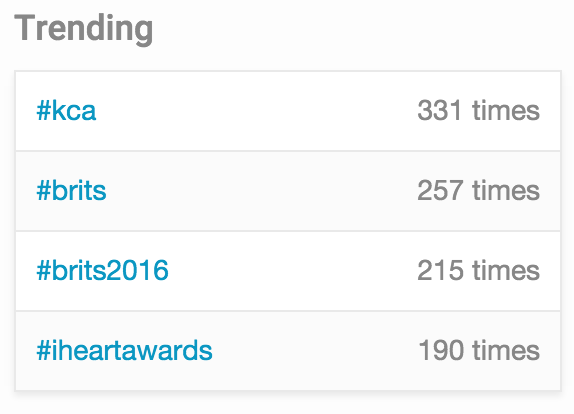
\includegraphics[scale=0.75]{trending.png}
\caption{The trending hashtags component. This screenshot was taken during the 2016 BRIT awards and the Kids Choice Awards.}
\label{trending}
\end{figure}
                       
    \subsection{HTTP Interface}
    Using the Play Framework, we expose an interface that the client side of the application can interact with. This interface consists of HTTP endpoints which can instruct the server to store or retrieve data from the model layer, or to open up a new channel (see Section 4.1.5). The endpoints available to the client are shown in Listing \ref{endpoints}.
    
\begin{lstlisting}[label=endpoints,caption=The exposed interface of the server.]
GET     /
GET     /ws/query/:queryString                      
GET     /ws/user/:screenName                        
GET     /ws/main/                      
GET     /learning/timeline/:screenName              
POST    /learning/rate-user                         
GET     /learning/get-user-relevance                
\end{lstlisting}

Each of these URLs are mapped to an associated method defined within a Play Framework Controller. By sending a request of the appropriate type to these endpoints, the client can interact with the server. The first defined endpoint (``GET /'') returns a sparse HTML document which contains a mount point. The client side renders the application's user interface inside this mount, as shown in Listing \ref{routerdef}.

                          
\section{Client Implementation}
The implementation of the client made use of several software development tools and practices which aimed to ease the development process. As described in Chapter 3, the front-end is constructed as a single page application which relies heavily on AJAX (Asynchronous JavaScript and XML) and WebSockets to efficiently fetch updates from the server, using those endpoints defined in Listing \ref{endpoints}.

        \subsection{Tools \& Practices}
        A number of tools were used on the front-end to assist in the design and build processes.
           
        \subsubsection{LESS}
        \textit{LESS} is a compiled superset of CSS (Cascading Style Sheets) which introduces a number of additional features including variables, nested definitions, and a module/import system \cite{less}.
        
        \subsubsection{CSS Flexbox}
        \textit{Flexbox} is a W3C specification for laying out elements within some parent element \cite{flexbox}. The majority of user interface elements used in ``Who To Follow In Context'' are built specifically for this project rather than from an external component library, and Flexbox was used extensively to align child elements within these components.

        \subsubsection{CommonJS Modules}
        \textit{CommonJS} introduces a module system into JavaScript/TypeScript \cite{commonjs}. As a result, it avoids the need to add one script tag to our index HTML page for each TypeScript file created. During the compilation step, the dependency tree of the front-end application is scanned and bundled into a single file.

        \subsubsection{Gulp}
        \textit{Gulp} is a front-end build system which was used to speed up parts of development \cite{gulp}. Gulp tasks were defined to watch TypeScript files for changes and automatically transpile them into new JavaScript files using the ``tsc'' TypeScript compiler. A Gulp task was also used in order to compile LESS files to CSS so that they could be interpreted by browsers.
        
        \subsubsection{Node Package Manager}
        \textit{Node Package Manager} (NPM) was used to manage front-end dependencies \cite{npm}. By specifying these dependencies in a \code{package.json} file, developers can simply run \code{npm install} to fetch all of the requirements for the application. NPM was used in conjunction with the \textit{TypeScript Definition Manager} which fetches TypeScript type declaration files.
        
        \subsection{User Interface}
\begin{figure}
\centering
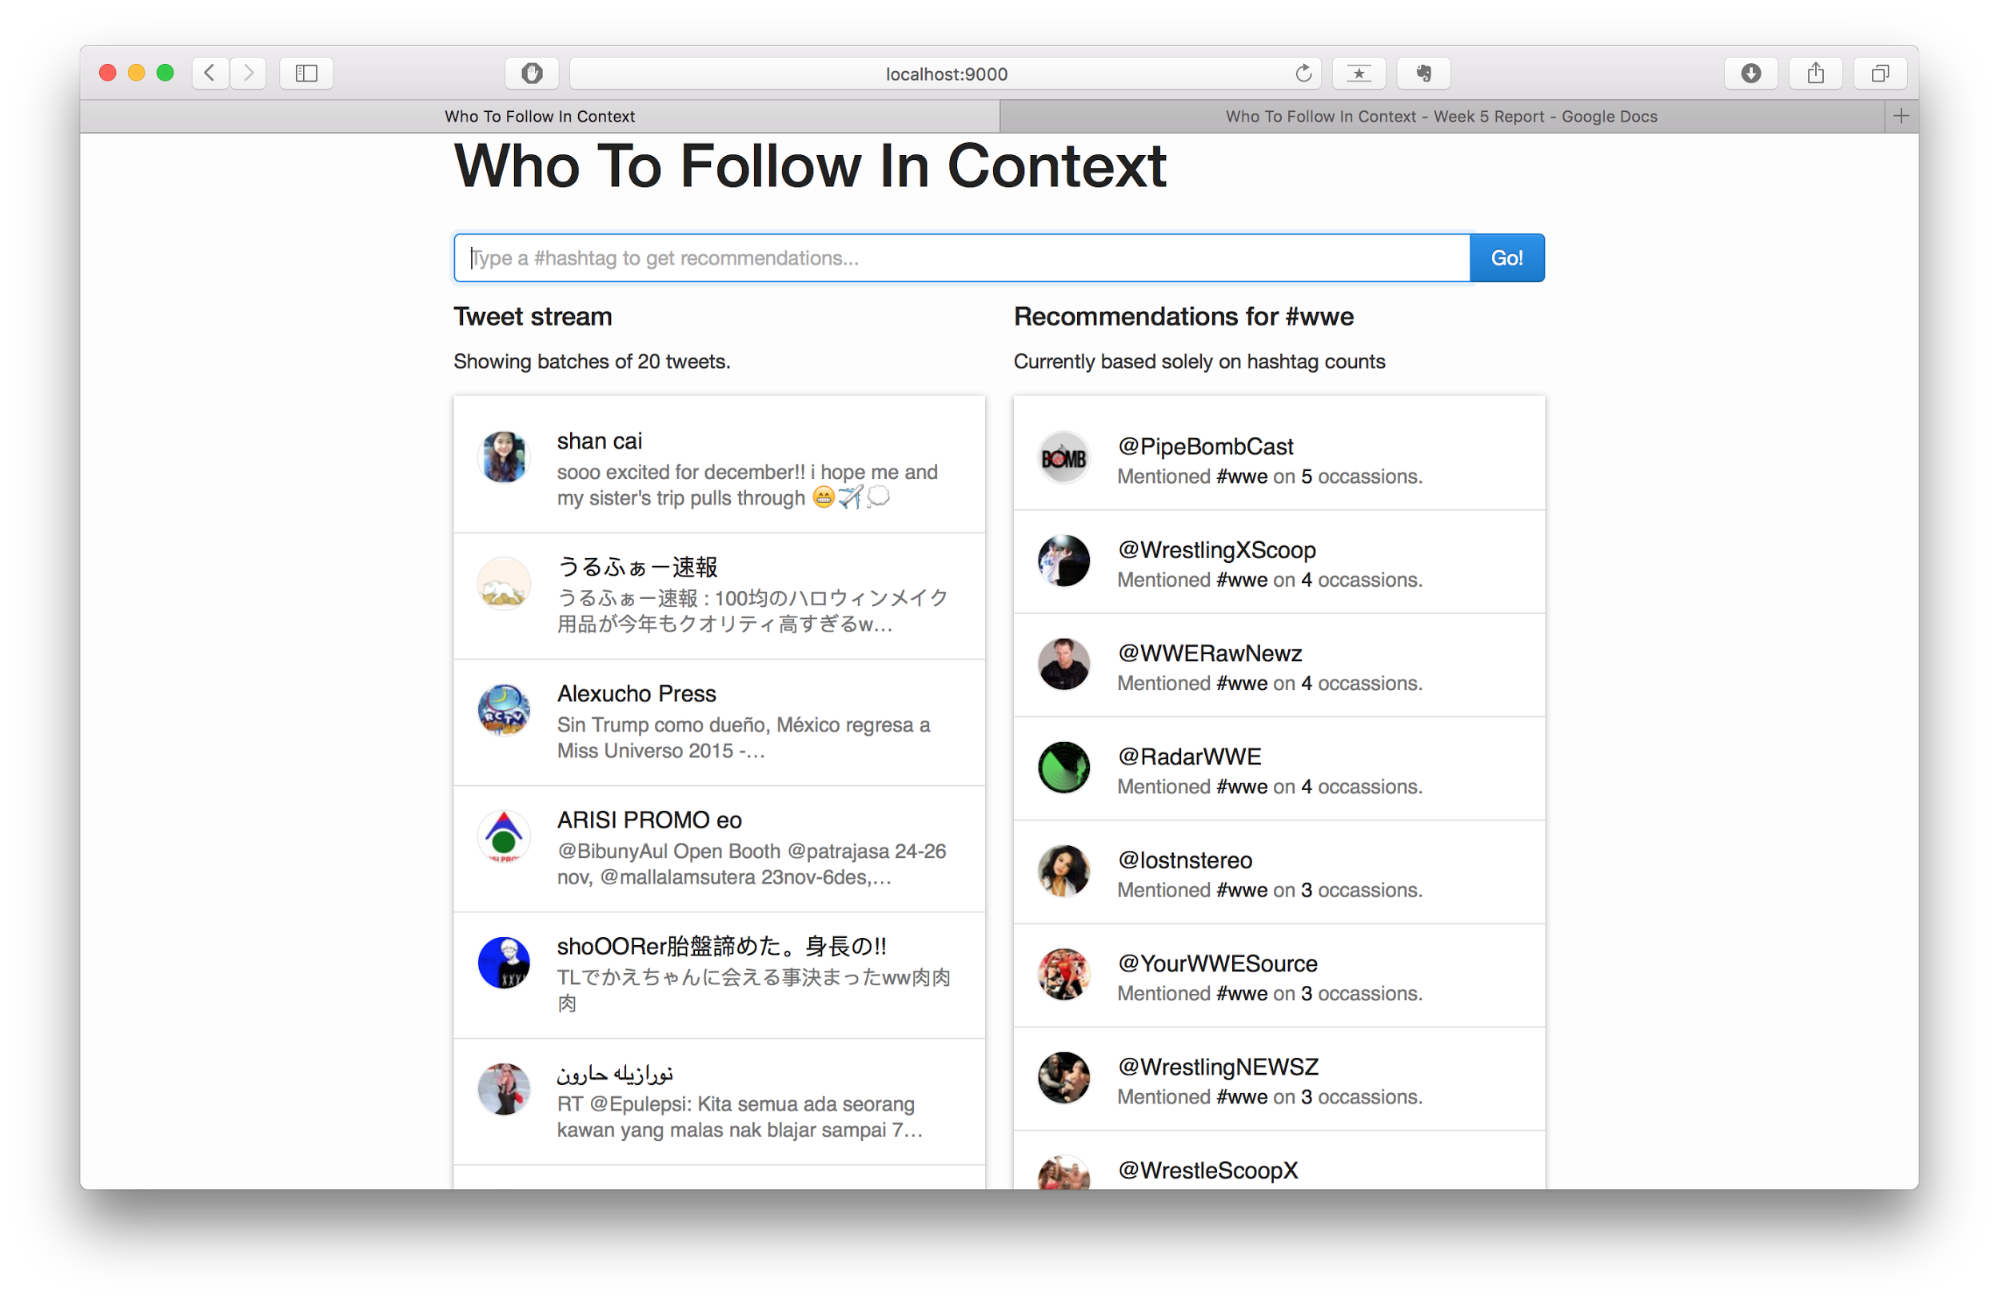
\includegraphics[scale=0.24]{initialui.png}
\caption{An early user interface prototype.}
\label{initialui}
\end{figure} 

        The user interface was one of the most heavily iterated upon aspects of the application. Using a component-based user interface library (React) allowed components to be iterated on in isolation, and so changing the UI could be done gradually to allow for progress on other features.
        
        An early proof of concept of the user interface (show in Figure \ref{initialui} displayed the stream of incoming tweets on the left half of the window, and the recommendations for the current query on the right hand side. After creating the proof of concept, mockups of several different UI components were created. An example of those created for the user suggestion components is shown in Figure \ref{suggestionsmockups}.
        
\begin{figure}[H]
\centering
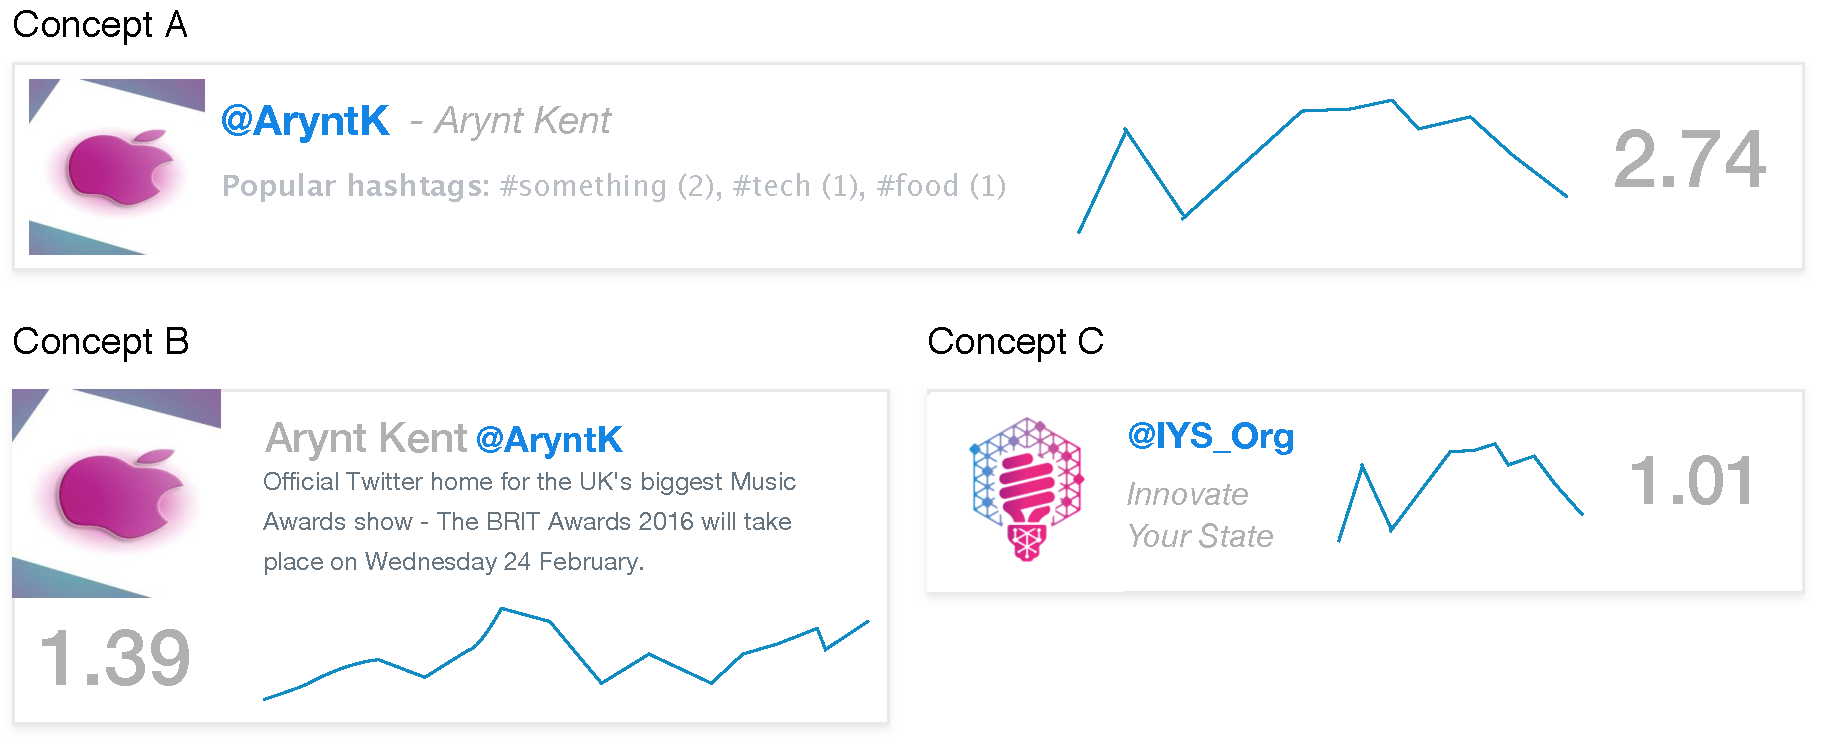
\includegraphics[scale=0.5]{suggestionsmockups.pdf}
\caption{Initial designs for the user suggestions components. In the final iteration of the UI, a modification of Concept C was used.}
\label{suggestionsmockups}
\end{figure}
        
        The initial mockup design of the ``Trending'' and ``Recent Searches'' lists is shown in \ref{listmockups}. These mockups were iterated on and eventually the front-end components were written in React to closely resemble them. The ability to view user timelines was not included at this point.
        
\begin{figure}[H]
\centering
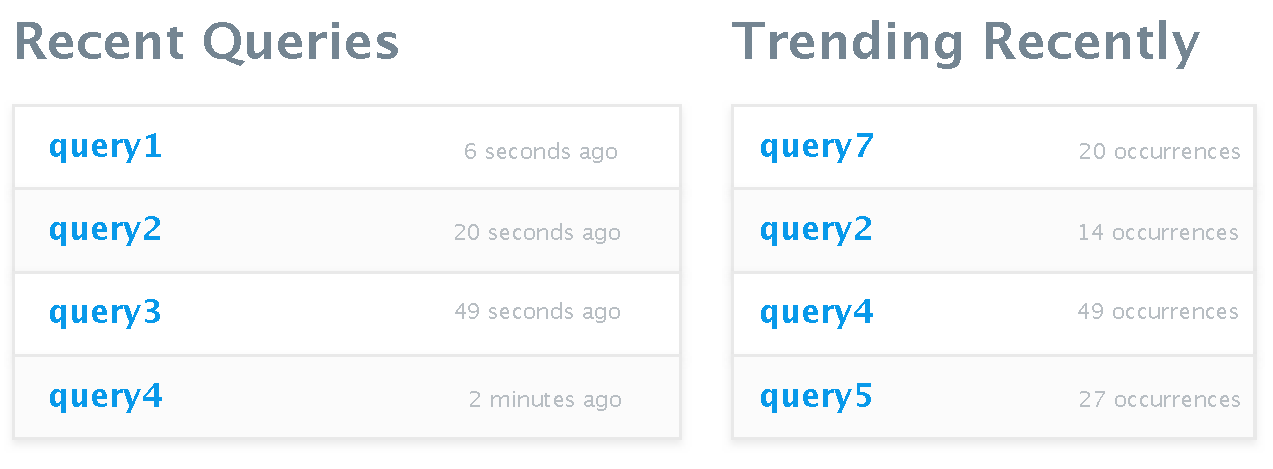
\includegraphics[scale=0.5]{listmockups.pdf}
\caption{The mockups created for the ``Recent Searches'' and ``Trending'' lists seen at the top right of the final UI in Figure \ref{finalscreenshot}.}
\label{listmockups}
\end{figure}    

After multiple iterations and further refinement of the project requirements, the final version of the user interface was created (see Figure \ref{finalscreenshot}).
        
\begin{figure}[H]
\centering
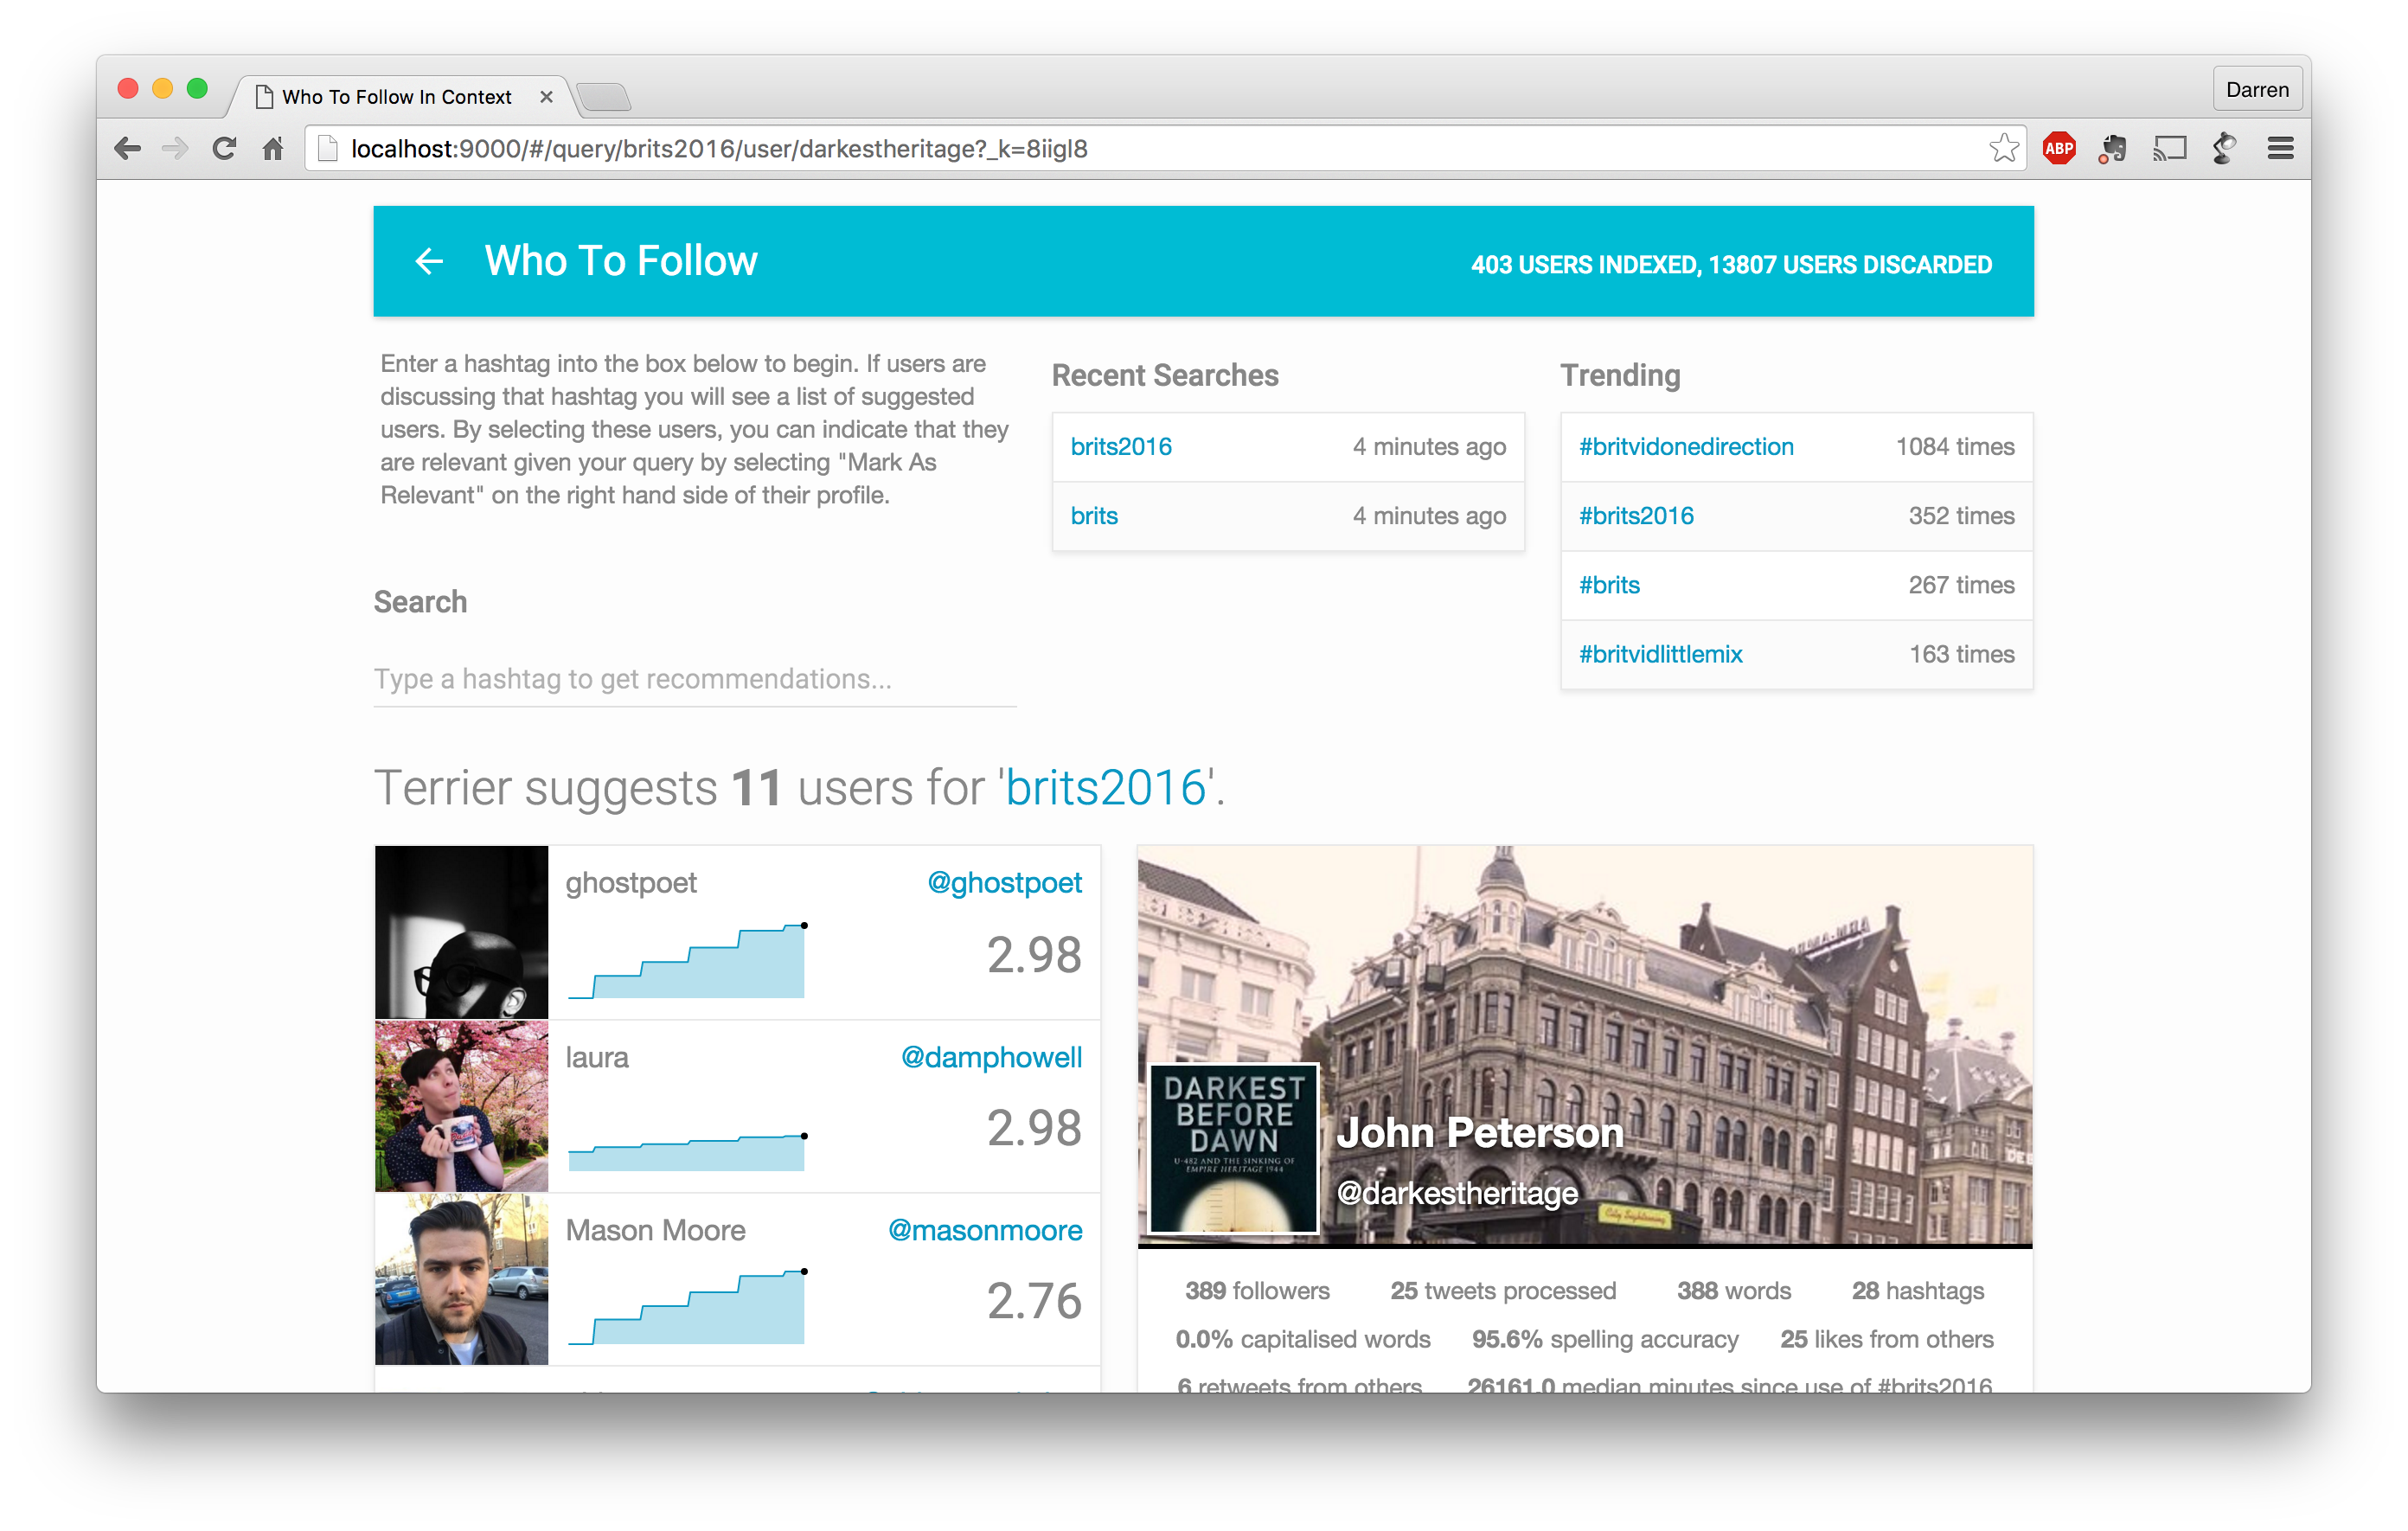
\includegraphics[scale=0.17]{finalscreenshot.png}
\caption{The final iteration of the user interface.}
\label{finalscreenshot}
\end{figure}

The final user interface consists of a search box shown on the left side of the display. By entering a query into this box and pressing ``enter'', a list of suggestions will appear underneath. These suggestions, as explained previously, update in real-time. This is to model the evolving nature of the live events they are providing suggestions for. By selecting a user in the list, we display a preview of the user's Twitter timeline. At the top right hand corner of the screen, we display real-time lists of ``Recent Searches'' and ``Trending Hashtags'', which exist to provide suggestions of queries that users may wish to enter.

    As discussed in the previous chapter, the user interface is implemented using a library called React. React allows user interfaces to be implemented using an extension of the syntax of JavaScript known as JSX, which is similar to XML. This syntax is compiled back into standard JavaScript in order to be parsed and executed by web browsers. The ``tsc'' TypeScript compiler comes with a built-in JSX compiler, and this was used by enabling it in TypeScript configuration file (\code{tsconfig.json}). This configuration is shown in Listing \ref{tsconfig}.
    
\begin{lstlisting}[label=tsconfig,caption=TypeScript compiler configuration.]
{
  "compilerOptions": {
    "jsx": "react",
    "module": "commonjs",
    "target": "es5",
    "allowJs": true
  },
  "exclude": [
    "node_modules"
  ]
}
\end{lstlisting}

By using the ``.tsx'' file extension, we inform ``tsc'' that the file contains JSX as well as TypeScript code, and that it must compile both of these syntaxes to plain JavaScript. An example of a React component which is written using TypeScript and JSX is shown in Listing \ref{tsjsx}. This component defines an individual item in a list, such as the ``Recent Searches'' and ``Trending'' lists. The component is defined generically, and is therefore written once, and reused in both of these lists.

\begin{lstlisting}[caption={Definition of a reusable list-item component using React, JSX, and TypeScript},label=tsjsx]
export class ScrollingListItem 
    extends React.Component<ScrollingListItemProps, any> {

    constructor(props) {
        super(props);
    }

    render() {
        return (
            <div className="scrolling-list-item" key={this.props.key}>
                <Link to={this.props.link}>
                    <span className="scrolling-list-item-text">{this.props.text}</span>
                </Link>
                <span className="scrolling-list-item-subtext">{this.props.subtext}</span>
            </div>
        )
    }

}
\end{lstlisting}

This component does not contain any internal state. Instead, it simply receives data from its parent component in the view hierarchy, and is tasked with displaying it. By keeping components stateless, they are more generic, and therefore more reusable. Writing reusable code in this way assists in satisfying requirement \textbf{N.5}, which says that the application must be constructed in a maintainable manner.

        \subsection{Searching}
        When a user enters a hashtag $Q$ into the search box and presses enter, an event handler is fired which changes the URL to \code{/\#/query/Q}. Since we are using React Router, the hierarchy of components mounted on the screen relates directly to the current URL. The TypeScript/JSX code which defines this hierarchy of components and their associated URLs is shown in Listing \ref{routerdef}.
        
\begin{lstlisting}[caption=Definition of the hierarchy of React component and how they map to the URL.,label=routerdef]
ReactDOM.render((
    <Router>
        <Route component={App}>
            <Route path="/" component={Home}>
                <Route path="/query/:query" component={QueryResults}>
                    <Route path="/query/:query/user/:screenName" component={TwitterUserPreviewPane} />
                </Route>
            </Route>
        </Route>
    </Router>
), document.getElementById("wtfc-app-mount"));
\end{lstlisting}
         
As a result of the code above, any requests to a URL beginning with \code{/\#/query} results in the \code{QueryResults} component and all of its parents to be mounted. In this way, all routing logic within the application is handled by the client. Immediately as \code{QueryResults} mounts, React calls its \code{componentDidMount} method, shown in Listing \ref{code:setquerychannel}. Inside this method, we send a request to the server to start the WebSocket handshake, and the server will create the channel for this query. In addition, we register callback functions which will execute when the client receives data from the server through the connected WebSocket, and the keep-alive messages that the client will send to the server for as long as \code{QueryResults} remains mounted. The TypeScript code which handles this process is shown in Listing \ref{code:setquerychannel} (extracted from the file \code{QueryResults.tsx}).

\begin{lstlisting}[caption=The method called by React when a new component mounts.,label=code:setquerychannel]
    componentDidMount: function() {
        // Creates WebSocket, keep-alive scheduled, registers callbacks
        this._setQueryChannel(this.props.params.query);
    },


    _setQueryChannel(query: string): void {
        let querySocket = new WebSocket(`ws://localhost:9000/ws/query/${this.props.params.query}`);
        querySocket.onmessage = event => {
            let recs: Array<UserScore> = JSON.parse(event.data)['results'];
            let actualResultSize: number = JSON.parse(event.data)['totalResultSize'];
            let history: Map<string, List<number>> = this.state.queryUserHistories;
            // Update the history for the graph for this user
            recs.forEach((rec: UserScore) => {
                let screenName: string = rec.screenName;
                if (history.has(screenName)) {
                    let userData: List<number> = history.get(screenName);
                    history = history.set(screenName, userData.push(rec.score));
                } else {
                    history = history.set(screenName, Immutable.List([]));
                }
            });
            this.setState({
                queryComplete: true,
                actualResultSize: actualResultSize,
                queryResults: Immutable.List(recs),
                queryUserHistories: history
            });
        };
        // Schedule keep-alives only after handshake complete
        querySocket.onopen = (event) => {
            // Continuously send Keep-Alives to inform server that we still want recs and stats
            let keepAlive = ChannelUtility.buildKeepAlive(this.props.params.query);
            querySocket.send(keepAlive);
            let keepAliveTrigger = setInterval(() => {
                Logger.info(`Sending keep-alive to query channel ${query}`, "KEEP-ALIVE");
                querySocket.send(keepAlive);
            }, Configuration.KEEP_ALIVE_FREQUENCY);
            this.setState({
                querySocket: querySocket,
                keepAlive: keepAliveTrigger
            });
        }
    },

\end{lstlisting}
        
        \subsection{Query Results}
        Query results are presented as a list on the left hand side of the display. Figure \ref{queryresults} shows how the query results are displayed. As the score for each user is re-evaluated, the ordering of the results changes. The numbers shown on the right hand side of the suggestions represent the users relevance score. The graph shown on each suggestion shows the historical changes in score for the corresponding user.
        
\begin{figure}[H]
\centering
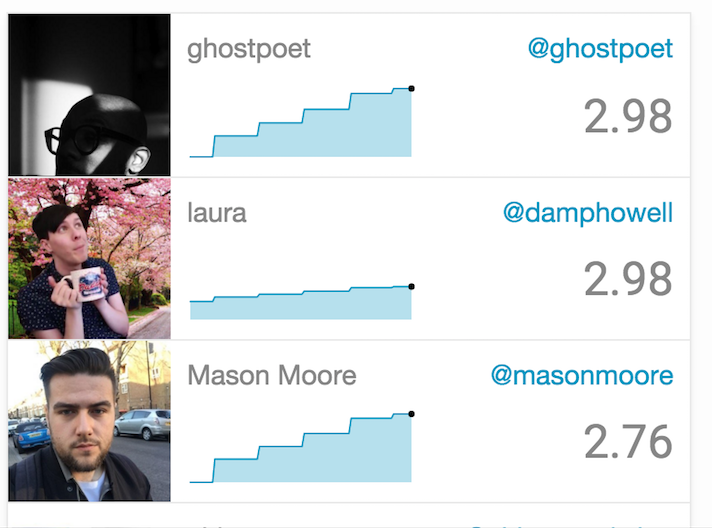
\includegraphics[scale=0.9]{queryresults.png}
\caption{An example of the display of suggested users.}
\label{queryresults}
\end{figure} 
        
        \subsection{Encouraging Interaction}
        At the top right hand corner of the screen we display real-time lists of the latest queries which have been entered by users of the system. We also display the most popular hashtags found within the past 10 minutes of streaming. The aim of these components is to encourage users to interact with the system by providing them with up-to-the-moment information on what is popular on Twitter and what users are currently searching for. By selecting an item in the list, it is entered as a query. It was hoped that this feature would make people more likely to interact with the system, since it may provide them with suggestions for hashtags they could search for. As discussed in the Evaluation chapter of this report, users said that these features did indeed make them more likely to interact with the application.
        
        \subsection{Previewing Twitter Users}
        On selecting a suggested account, users are shown a preview of that account without having to leave the application. Figure \ref{userpreview} shows how we display the preview to users. Several elements of this view are personalised for each user, taking into consideration the colours used in their Twitter profile. Any occurrences of the query term within tweets are highlighted to bring attention to potentially relevant tweets. By previewing the suggestion within the application, users can provide relevance feedback for the purposes of evaluation and improving the relevance of future query results. This component fades into view, to prevent confusion that may be caused in the case that another user was being viewed and is immediately replaced by a new user. This animation was created using \textit{Velocity-React}, which allows animations to be specified declaratively \cite{velocityreact} using JSX syntax.
        
\begin{figure}
\centering
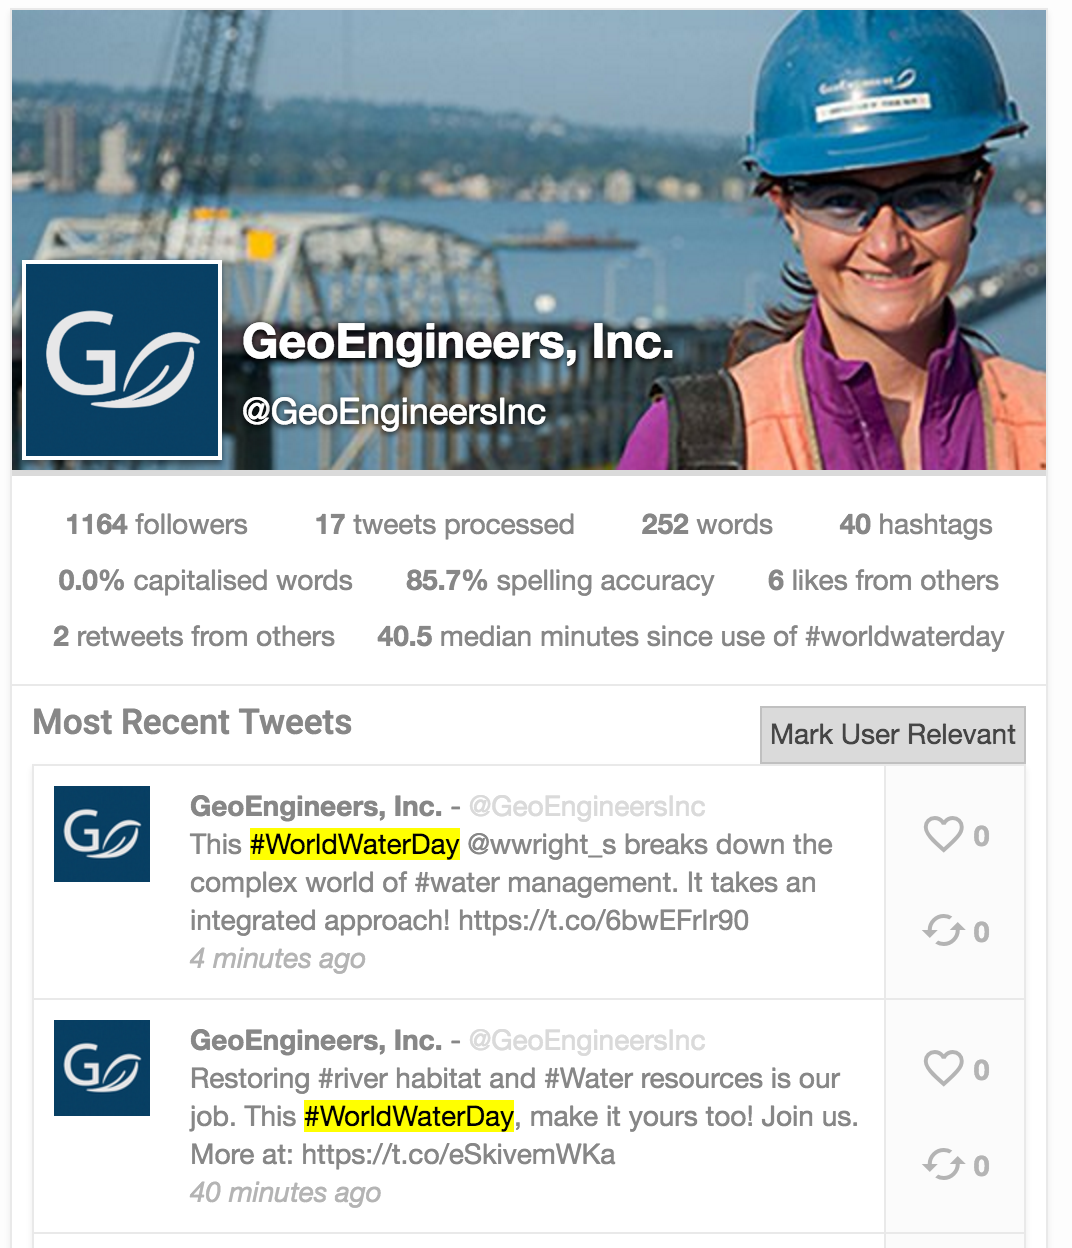
\includegraphics[scale=0.5]{userpreview.png}
\caption{The preview of a user's Twitter profile that is shown when a suggestion is selected.}
\label{userpreview}
\end{figure}         
        
        
    \section{Summary}
    Both client and server presented a number of implementation challenges. This chapter has described some of these challenges and how they were overcome. On the server it was shown how feature extraction, indexing, and retrieval were performed. The use of real-time technologies such as the use of WebSockets to implement channels was also discussed. A variety of techniques for improving system responsiveness such as asynchronous programming, and actor pooling were also described.
    
    In the description of the implementation of the client side, the use of a single page application and client side routing were explained. Early prototypes of the user interface were shown, and then the final iteration of the user interface was displayed, and its components were described.        
        
        
\chapter{Evaluation}

After implementation had concluded, the application was evaluated using a variety of different evaluation techniques. The purpose of this evaluation was to attempt to answer the following questions:

\begin{enumerate}
\item Is there a gap in the market for this product?
\item Did users find the system to be usable?
\item Did the system help users find Twitter users with expertise in ongoing events?
\item What impact on results and the number of users discarded do different filtering configurations have?
\item What is the impact of altering the rate at which the system reads tweets?
\end{enumerate}


\section{User Evaluation}

    In addition to weekly feedback from the project supervisor, a user evaluation study was conducted in the final weeks of the project to determine users opinions on the application.

    \subsection{Questionnaires}
    Two separate questionnaires were used. The first aimed to gain insight into how people use Twitter, and the second was a post-evaluation questionnaire enabling them to provide additional feedback after the think-aloud session.
    
        \subsubsection{Twitter Usage Questionnaire}
        This questionnaire was distributed to a subset of Level 4 Computing Science students at the University of Glasgow. 18 students completed this questionnaire. The intention was to determine how people use Twitter, specifically in the context of events. It also aimed to discover what motivates them to use Twitter and the considerations they make before following users. By gaining insight into these areas, we can gain a better understanding of the difficulties that Twitter users have, allowing us to determine whether there exists a gap in the market for this product.

\begin{enumerate}

\item \textit{How often do you use Twitter?}
\par
\begin{figure}[H]
\centering
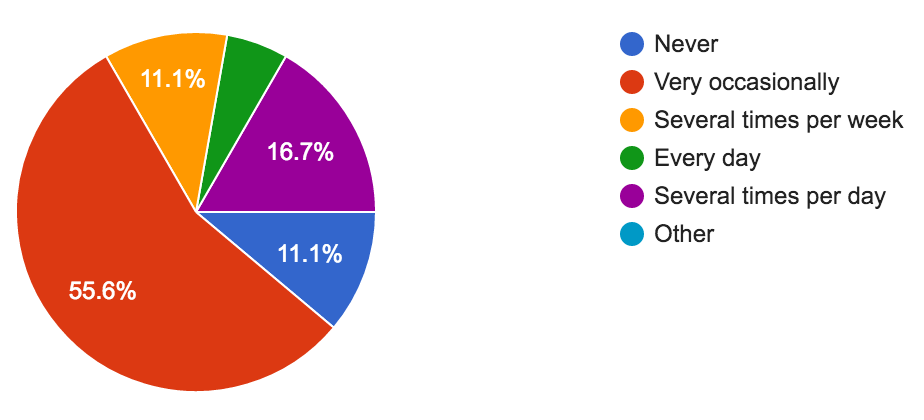
\includegraphics[scale=0.7]{howoftentwitter.png}
\label{howoftentwitter}
\end{figure}
The majority of respondents said that they use Twitter less than once per week (labelled as \textit{Very occasionally}). Additionally, 11\% of respondents said that they never use Twitter, but have used it in the past and so understand its concepts.


\item \textit{How many people do you follow on Twitter?}
\par
Participants in the survey follow on average 150.2 Twitter users. Two respondents gave an approximation of the number of people they followed, and one respondent who no longer uses Twitter said they follow zero users. As a result, this figure is likely to be slightly below the true value.

\item \textit{Approximately what proportion of tweets that you see on Twitter do you find to be relevant to your interests?}
\par
\begin{figure}[H]
\centering
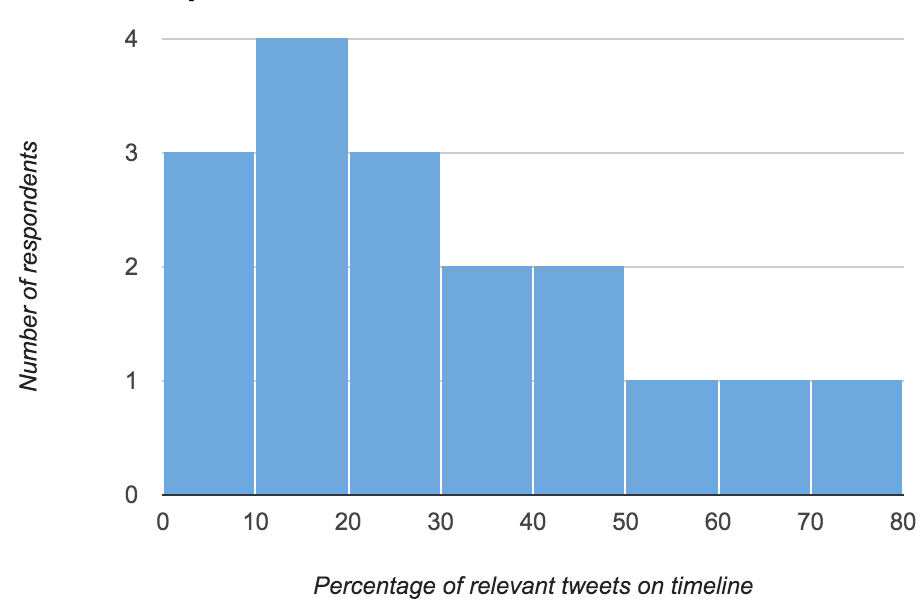
\includegraphics[scale=0.5]{proprelevance.png}
\label{proprelevance}
\end{figure}
This question aimed to determine how well Twitter currently does at meeting the information needs of users. The results showed that users generally find a minority of the information they see on Twitter as relevant to their interests, with over two thirds of participants saying that they believe less than 50\% of the content they see is relevant.

\item \textit{What considerations do you make when you decide to follow someone on social media?}
\begin{table}[H]
    \centering
    \begin{tabular}{| l | l | l |}
    \hline
    Consideration & Number of agreements & Percentage (\%) \\ \hline
    Their popularity & 5 & 27.8  \\ \hline
    How often they tweet & 3 & 16.7 \\ \hline
    The contents of their tweets & 16 & 88.9 \\ \hline
    Whether you know them in real life & 10 & 55.6 \\ \hline
    Whether following them is appropriate & 4 & 22.2 \\
    \hline
    \end{tabular}
\end{table}
The majority of respondents (88.9\%) said that the the contents of the tweets written by users is one of the considerations they make when deciding whether to follow them or not. Only 27.8\% of respondents said that they consider the popularity of the account, despite this being one of the main signals used by existing services in the ranking of accounts. As such, this may be an indication that the current content-based approach to suggesting accounts to follow is more in line with what users want.

\item \textit{How easy do you find it to discover people tweeting about ongoing events?}
\par
\begin{figure}[H]
\centering
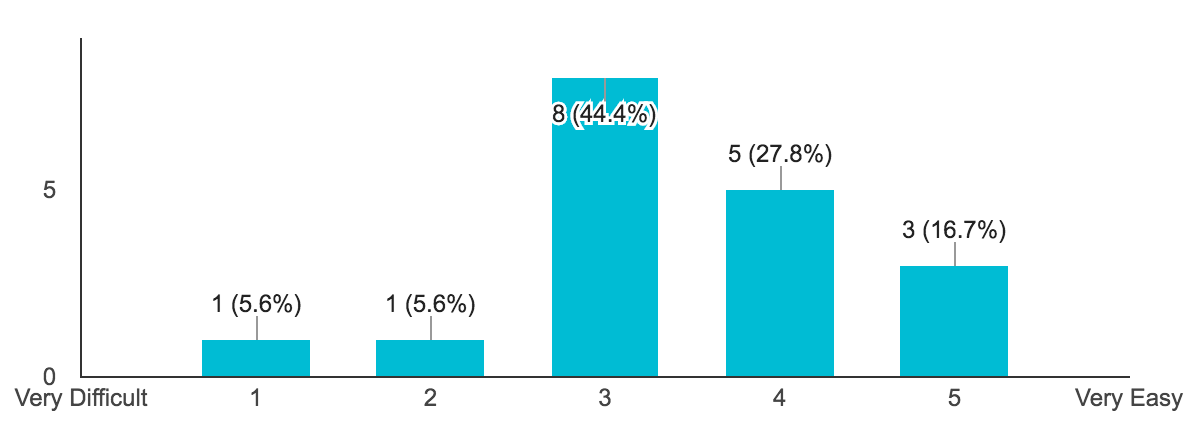
\includegraphics[scale=0.7]{findingusers.png}
\label{findingusers}
\end{figure}
Participants in general found it relatively simply to find users tweeting about ongoing events.


\item \textit{How easy do you find it to discover people tweeting \textbf{frequently} about ongoing events?}
\par
\begin{figure}[H]
\centering
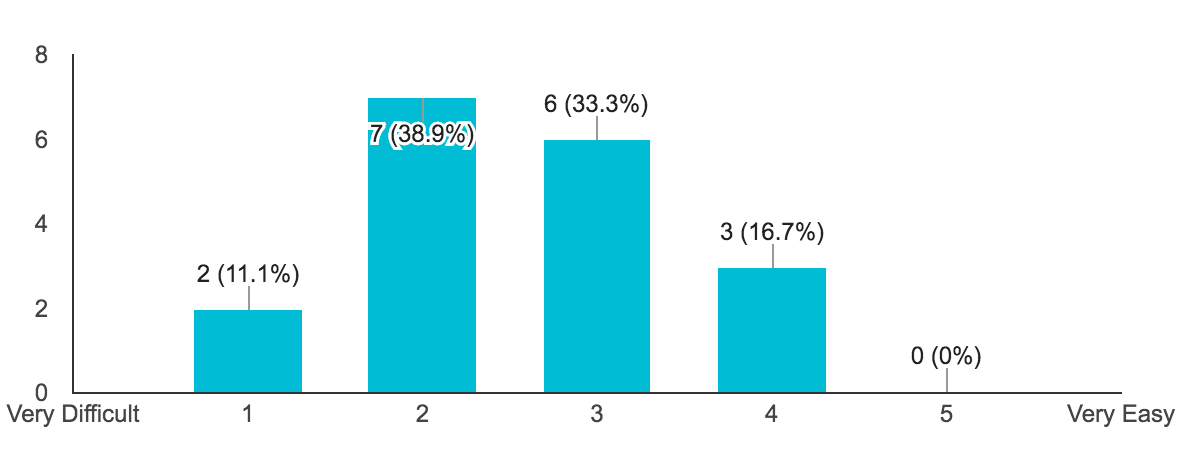
\includegraphics[scale=0.7]{findingusersfreq.png}
\label{findingusersfreq}
\end{figure}
When tasked with finding users who are frequently tweeting about an ongoing event, particpants say they have more difficulty. The results are skewed towards \textit{Very difficult}, in contrast with question 5. This suggests that Twitter's existing product has been relatively unsuccessful  at assisting people in meeting their need for expertise with regards to events.

\item \textit{Do you believe you would use Twitter more if you followed more people you are interested in?}
\par
\begin{figure}[H]
\centering
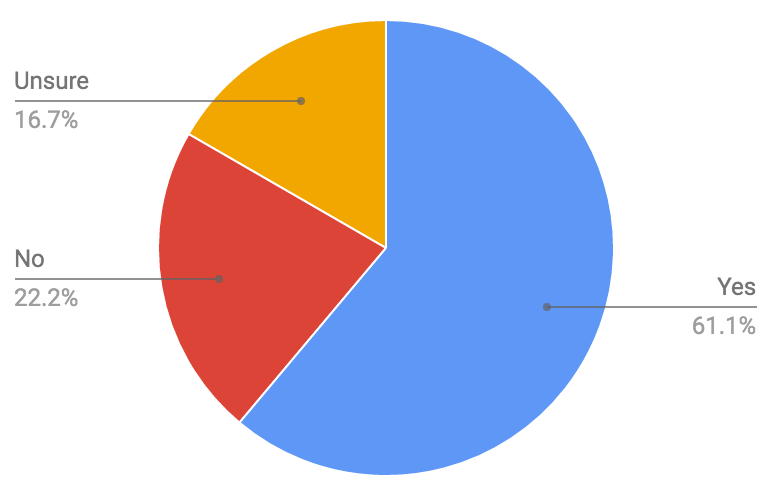
\includegraphics[scale=0.55]{usetwittermore.png}
\label{usetwittermore}
\end{figure}
The majority of questionnaire respondents said that they would use Twitter more if they followed more people that they are interested in. This suggests that recommending users which meet the information needs or interests of users is likely to increase the amount of time that people spend on Twitter.

\item \textit{I am more likely to use Twitter if an event I am interested in is currently happening. (1 represents strongly disagree, 5 represents strongly agree)}
\par
\begin{figure}[H]
\centering
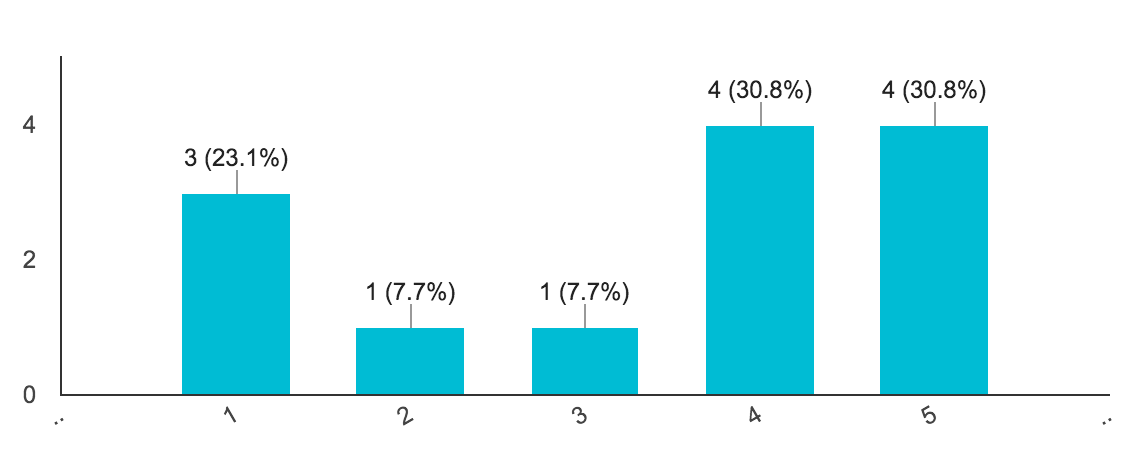
\includegraphics[scale=0.55]{morelikelytwitter.png}
\label{morelikelytwitter}
\end{figure}
This question aimed to determine the influence that ongoing events have on peoples decision to visit Twitter. A majority of respondents replied saying that they either ``Agree'' or ``Strongly Agree'' that ongoing events that they have an interest in increase the likelihood of them visiting Twitter.



\end{enumerate}


The results of this questionnaire show that Twitter users have issues with the existing services which are similar to this project. In particular, they struggle to recommend users who have been frequently discussing ongoing events, despite a large number of respondents saying that such events make them more likely to use Twitter. This would suggest that there is indeed a gap in the market for this product, targeting the subset of the population which use Twitter to follow ongoing events.
               
        \subsubsection{Post-Evaluation Questionnaire}
        The purpose of this questionnaire was to retrieve feedback from users after they have evaluated the project, and to attempt to answer evaluation questions 2 and 3 (listed at the start of this chapter). The questionnaire asked users for feedback on system usability, and for their opinion on the overall relevance of the suggestions. Participants were asked to answer questions on a scale from 0 to 9, where 0 represents ``strongly disagree'' and 9 represents ``strongly agree''. The results of the usability section of this questionnaire are shown in the Table \ref{table:posteval}.
        
\begin{table}[H]
    \centering
    \begin{tabular}{| l | l |}
    \hline
    Question & Mean Response \\ \hline
    Overall, I am satisfied with how easy it is to use this system. & 8.00 \\ \hline
    It was simple to use this system. & 7.83 \\ \hline
    I can effectively complete tasks using this system. &  7.66 \\ \hline
    I feel comfortable using this system. & 7.33 \\ \hline
    It was easy to learn to use this system. & 8.00 \\ \hline
    Whenever I make a mistake using the system, I can recover easily and quickly. & 7.66 \\ \hline
    The organisation of information on the screen is clear. & 7.83  \\ \hline
    The user interface of the system is pleasant. & 7.83  \\ \hline
    I like using the interface of the system. & 8.50  \\ \hline
    I believe the system kept me informed of what it was doing. & 6.00 \\ \hline
    I found that the system responded quickly to my actions. & 8.17  \\ \hline
    \textbf{Average} & \textbf{7.71} \\
    \hline
    \end{tabular}
    \caption{\label{table:posteval}The average responses from the usability section of the post-evaluation questionnaire.}
\end{table}

The project score an average of 7.71 out of 10 across all usability questions, indicating that users overall found the system to be usable. However, responses to individual questions indicate that there are certainly areas which can be improved. For example, increasing the level of feedback users receive when they perform actions may result in an improvement in mean response for the lowest scoring question (``I believe the system kept me informed of what it was doing'').

Participants were also asked to judge whether they were happy with more specific areas of the project, such as the suggestions made and the impact of individual elements of the user interface. The results from this part of the evaluation are shown in the Table \ref{table:posteval2}.

\begin{table}[H]
    \centering
    \begin{tabular}{| l | l |}
    \hline
    Question & Mean Response \\ \hline
    I believe that the updating ranks gave me insight new participants on discussions. & 7.17 \\ \hline
    I found the ranking of users suggested by the system to be accurate. & 6.33  \\ \hline
    I found the 'Trending' hashtags list encouraged me to use the system. & 7.50 \\ \hline
    I found the users suggested by the system to be relevant. & 7.00 \\
    \hline
    \end{tabular}
    \caption{\label{table:posteval2} Responses to remaining post-evaluation questions.}
\end{table}

The results from this section of the post-evaluation questionnaire suggest that users overall were relatively happy with the suggestions made by the system, giving it the suggestions an average score of 7. However, users were less satisfied with the ranking of these results, with a lower average response of 6.33. These scores suggest that the application did indeed assist users in finding users tweeting about ongoing events.
 
    \subsection{Think-Aloud Study}
    All six evaluation participants participated in a ``think-aloud'' study, whereby they speak their thoughts aloud as they interact with the application. The intention of this study was to determine whether the application had any significant usability issues that multiple users noticed, and to determine the size of the ``Gulf of Execution''. That is, we try to determine the extent by which the actions that users perceive as being required to complete the task and the correct actions required differ. The task given to the users was to try and find users that are currently tweeting about the 2016 BRIT Awards.
    
    A variety of constructive feedback was retrieved during these sessions. Some of the most common or constructive items of feedback are shown below.
    
\begin{itemize}

\item \textit{``The back button at the top left corner of the home-page when you first arrive on the application is confusing.''}
\par
Two participants noted that this button was confusing because they had just arrived on the site from elsewhere. The back button works identical to the browsers back button, so on first arrival it takes users back to the previous URL they visited (even if it wasn't within this application). It was suggested that this be replaced with a ``Home'' button.

\item \textit{``It wasn't immediately obvious that selecting a hashtag in the ``Trending'' or ``Recent Searches'' lists would submit a search for it.''}
\par
Although users generally said they were not surprised that selecting an item in the list performed a search when they tried clicking on it, it was generally felt that it could be made clearer exactly what would happen.

\item \textit{``When I search, it is not clear whether I have to include the hashtag symbol or not.''}
\par
Every participant made note of this, but it did not cause any issues because the application accepts either case.

\item \textit{``I assume that the graphs and numbers in user suggestions are some form of relevance score, but it is not completely clear.''}
\par
Participants were more confused about the graph than the scores (see Figure \ref{queryresults}). All of them understood that the score indicated some ranking function, but the idea that the graphs represent the change in each users score \textit{in isolation} caused confusion.

\item \textit{``It would be nice if I could access someones Twitter easily from the application so that I can follow those accounts that I find interesting.''}
\par
This feature was present in an older version of the product, and it was an oversight that it was not added to the current iteration.

\item \textit{The trending hashtags encouraged interaction as intended - users ended up making several additional searches by selecting items in this list.}

\item \textit{Most users completely ignored the help text provided.}

\end{itemize}

The information gathered from the think-aloud sessions show that there are certainly areas of the application that can be improved on from a usability perspective. However, there were no critical issues discovered, and the overall feedback received was positive (as shown previously in Table \ref{table:posteval}).

\section{Experiments}

Two experiments were performed with the system. The first examined filtering controls, the second examined the impact of altering the rate at which the system reads tweets. These were intended two answer evaluation questions 4 and 5 respectively. 
    
    \subsection{Experimenting With Filtering Controls}
    The implications of altering the threshold at which tweets are discarded during the filtering stage were examined in order to answer evaluation question 4. It was hypothesised that the ``Spelling Accuracy'' and ``Follower Count'' filters would have the largest impact on the number of users discarded. By altering this configuration, the effect of filtering on the number of users the application has to process was investigated. Using the default filtering controls shown in Table \ref{table:standardfilters}, it was found that in a sample of 15000 tweets, approximately $97\%$ of users were discarded at the filtering stage. This shows that the combination of seemingly relaxed filters can result in a large number of users being dropped and therefore massively reducing the load on the server. 
    
Further experiments were performed to determine the impact that the individual default filters have on the overall number of users filtered. This experiment was performed by disabling all user filtering, and examining the effects of individual filters by applying them in isolation. The determined contribution of the individual default filtering controls is shown in Table \ref{table:filteringresults}. The total percentage of users filtered is greater than 100\% because a single tweet will usually fail the checks imposed by several filters at once.

\begin{table}[H]
    \centering
    \begin{tabular}{| l | l |}
    \hline
    Filter Name & \% of Users Filtered \\ \hline
    ALL FILTERS & 97 \\ \hline
    Spelling Accuracy & 92  \\ \hline
    Follower Count & 44 \\ \hline
    Word Count & 30 \\
    \hline
    \end{tabular}
    \caption{\label{table:filteringresults}The individual impact of different filtering controls. ($N=15000$).}
\end{table}

Three participants repeated the practical evaluation using the system under a modified set of filtering controls. The modified controls were identical to the default controls shown in Table \ref{table:standardfilters}, except the ``follower count'' filter was completely removed. As a result of this, the additional 44\% of users with less than 300 followers are processed. The participants who examined this modified configuration all said that a significantly larger number of suggestions were made by the application. They also said that there was very little noticeable difference between the quality or relevance of the results when comparing the two configurations. This may indicate that the ``Follower Count'' signal should not be weighted so heavily when deciding which users to filter from the stream. This observation suggests that manual filter controls are difficult to properly tune without repeated evaluation. Therefore, using classification techniques based on machine learning may provide a more robust means of finding an optimal weighting to apply to filtering parameters.
    

   
\begin{table}
    \centering
    \begin{tabular}{| l | l | l |}
    \hline
    Filter Name & Required Value & Description\\ \hline
    Spelling Accuracy & $>50\%$ & Tweets with 50\% or less of words spelt correctly are discarded.  \\ \hline
    Word Count & $>3$ & Tweets with 3 or less words are discarded.  \\ \hline
    Follower Count & $\geq300$ & Tweets with authors who have less than 300 followers are discarded. \\ \hline
    Hashtag Count & $<5$ & Tweets with 5 or more hashtags are discarded. \\ \hline
    Capitalised Words & N/A & Tweet entirely capitalised are discarded. \\
    
    \hline
    \end{tabular}
    \caption{\label{table:standardfilters}The default filtering controls.}
\end{table}

    
    \subsection{Investigating the Effects of Stream Replay Rate}
    The rate at which tweets are read when using a source file has a direct effect on system performance and usability, in order to answer evaluation question 5. An investigation was conducted into the performance and usability impact of altering the \textit{stream replay rate}. The stream replay rate is the rate at which new tweets are read into the system from a source file. This rate is configurable using two parameters: ``BatchDuration'' and ``BatchSize'' (\textbf{Note}: these parameters are unrelated to the batching performed by Spark Streaming described in the ``Implementation'' chapter). The ``BatchDuration'' parameter defines the time between examining batches of tweets from the source. The ``BatchSize'' parameter defines the number of tweets in each of these batches. These parameters can be configured using the file entitled ``application.conf'', and are shown in Listing 5.1. Users were given the opportunity to perform tasks with the system with two different stream replay rates, and asked to provide feedback on which version they preferred. The replay rates that users evaluated are described in Tables \ref{table:replayrate1} and \ref{table:replayrate2}.
    
\begin{table}[H]
    \centering
    \begin{tabular}{| l | l | l |}
    \hline
    Parameter & Value & Description \\ \hline
    BatchSize & 70 & Each batch contained 70 tweets. \\ \hline
    BatchDuration & 1000 & A batch was processed every 1000 milliseconds. \\
    \hline
    \end{tabular}
    \caption{\label{table:replayrate1} The default stream replay configuration (70 tweets/sec, updating every second).}
\end{table}

\begin{table}[H]
    \centering
    \begin{tabular}{| l | l | l |}
    \hline
    Parameter & Value & Description \\ \hline
    BatchSize & 100 & Each batch contained 100 tweets. \\ \hline
    BatchDuration & 500 & A batch was processed every 500 milliseconds. \\
    \hline
    \end{tabular}
    \caption{\label{table:replayrate2} The modified stream replay configuration (200 tweets/sec, updating every half second).}
\end{table}     
    
\begin{lstlisting}[caption=Configuration of the stream replay rate in application.conf,language=Ini]
# path to gzipped json file containing tweets which will be read
# leave blank for live stream
stream.sourcefile.path = "/path/to/gzipped/tweets.json.gz"
# the number of tweets in each batch
stream.sourcefile.batchSize = 100
# time in milliseconds between each batch
stream.sourcefile.batchDuration = 500
\end{lstlisting}

Participants stated that they preferred the rate at which suggestions are made using the modified stream replay configuration. However, one person observed that for more popular events the faster update speed may make the user interface difficult to interact with. In reality, the optimal update rate is dependent on the popularity of the event. As such, it may be required in the future to buffer results on the client side for extremely popular events, giving users the ability to update them whenever they wish.

\section{Behaviour Testing}

    Testing was done using the \textit{Specs 2} Scala testing framework \cite{specs2}. This framework allows us to define how our application works in terms of its behaviours. Tests were written to examine feature extraction, querying, and the servers response to requests for the single page the application is mounted at. These tests worked in isolation, but the author was unable to configure the Play Framework in order to run all of the tests using the same application. It proved extremely difficult to configure the environment that the tests execute in to match the environment that the application runs in. As such, each Specs2 specification had to be run individually, using a separate Play application for each. Unfortunately, these issues proved cumbersome to work around, and so testing focuses primarily on critical areas of source code. Further work would be required in this area to resolve this issue. 
     
    Akka TestKit \cite{akka} made it possible test the direct output of the internal behaviour of actors by exposing the methods defined inside the actor. These methods are traditionally hidden by Akka. An example of how the internal behaviour can be examined is shown in Listing \ref{test}.
    
\begin{lstlisting}[label=test,caption={Testing the internal behaviour of an actor.}]
"A QueryService actor" should {

    "return an empty TerrierResultSet with an actual size of 0 on an empty query" in new Actors {
      running(app) {
        // Get the underlying actor (typically hidden by Akka)
        val queryServiceActor = TestActorRef(app.injector.instanceOf(
            BindingKey(classOf[QueryService]))
        ).underlyingActor
        // Check the response
        queryServiceActor.doQuery(EmptyQuery).actualSize must be equalTo 0
      }
    }
    
    ...
\end{lstlisting}
    
        
\section{Integration Testing}
    In addition to tests which ensure that components behave as expected, tests were also written to ensure that they work correctly within their intended environment. In the context of actor systems, this is done by testing how actors respond to \textit{stimulus} from a \textit{probe}. Since actors perform computation in response to messages, we can probe their behaviour by sending them test messages and ensuring that they respond as expected.
    
    As an example of how integration testing was useful: When a \code{SparkContext} has been started, it is illegal to attempt to register additional actions on the data. Since the system registers Spark actions in asynchronous calls, it is a possibility that the \code{SparkContext} is started before all actions are registered. To avoid this scenario, any actor registering Spark actions must inform its parent when it has done so. The parent will wait for all child actors to make this confirmation before starting the context. Integration testing is used to ensure that all actors which register Spark actions correctly inform their parent when this registration is complete, and thus avoids a runtime \code{IllegalStateException}. The associated test is shown in Listing \ref{integrationtest}.
    
\begin{lstlisting}[label=integrationtest,caption=Ensuring that the FeatureExtraction actor is correctly instantiated.]
"The FeatureExtraction actor should respond that it is ready when it receives a Twitter stream handle" in new Actors {
    running(app) {
      val featureExtractionActorRef = TestActorRef(app.injector.instanceOf(BindingKey(classOf[FeatureExtraction])))
      val probe = TestProbe()  // Construct the 'probe'
      val config = app.injector.instanceOf(classOf[Configuration])
      val streamPath = app.configuration.getString("stream.sourcefile.path").get
      val handle = SparkInit.ssc.actorStream[Status]
          (TweetStreamSimulator.props[Status](streamPath, 10, 10), TweetStreamSimulator.name)
      // Apply 'stimulus'    
      featureExtractionActorRef.tell(ActiveTwitterStream(handle), probe.ref)
      // Ensure correct response is received within 10 seconds
      probe.expectMsgType[PipelineActorReady](FiniteDuration(10, TimeUnit.SECONDS))
    }
  }
\end{lstlisting}    

    \section{Summary}
    Throughout this chapter, we have attempted to answer the evaluation questions listed at the beginning of the chapter. These answers are summarised below.
    
\begin{enumerate}
\item \textit{Is there a gap in the market for this product?}
\par
Through the findings of the Twitter usage questionnaire, it was determined that there is indeed a market for the product. The findings of this questionnaire were discussed in detail in Section 5.1.1.
\item \textit{Did users find the system to be usable?}
\par
The application scored an average of 7.71 out of 9 in response to the usability questions posed in the post-evaluation questionnaire, indicating that users did find the system to be usable. These responses were discussed in Section 5.1.1.
\item \textit{Did the system help users find Twitter users with expertise in ongoing events?}
\par
The second set of questions within the post-evaluation questionnaire indicated that users were overall happy with the results provided by the system, but it was found that there is certainly room for improvement. (See Section 5.1.1 - Post-Evaluation Questionnaire)
\item \textit{What impact on results and the number of users discarded do different filtering configurations have?}
\par
Section 5.2.1 showed that altering the filtering configuration can have a large impact on the number of users filtered. It showed that some filters have a disproportionally large impact on the number of users discarded. It was found that there was little difference between the filtering configuration which discarded accounts with less than 300 followers, and the configuration that didn't.

\item \textit{What is the impact of altering the rate at which the system reads tweets?}
Section 5.2.2 examined the impact of altering the ``stream replay rate''. It was found that given the two test configurations, users enjoyed using the faster configuration (200 tweets/sec, updating every half second) more. However, it was noted that for extremely popular events, updating the display every half second may cause difficulty.
\end{enumerate}
    

\chapter{Conclusion}

    The final iteration of the ``Who To Follow In Context'' product implements a majority of the project's requirements. The project can analyse a stream of tweets in real-time, from either a source file or the Twitter live streaming API, and display dynamic results to users.
    
     The architecture of the product has been thoroughly documented in this report, and the implementation of several of its components has been discussed in detail. The functions of these components ranged from processing a stream of tweets to handling concurrent queries submitted from several users. The development of the user interface was also discussed, as well as several implementation challenges and design decisions that were associated with it. In particular, the decision to construct the application as a single-page application was of note, since it involved the unusual decision of delegating URL routing logic to the client-side. The benefits of such an architecture were discussed in the Implementation chapter.
    
     During the evaluation it was shown that this analysis can be performed without a noticeable impact on the responsiveness of the user interface. It has also been shown that users are overall happy with the usability of the final product, and the quality of the suggestions that it makes. Evaluation work also suggested that there is a segment of the market suffer from the problems which this application aims to solve. Finally, we found that removing a relatively impactful filter (follower count) had little to no impact on users perception of the quality of suggestions. The evaluation phase also proved extremely useful in discovering candidate ideas for future development.
    
    \section{Future Work}
    
    If work was to continue on the project, there are several areas which could be improved or extended. Some of these suggestions are made with the power of hindsight, whilst others are made as a result of the evaluation conducted in the previous section.
    
        \subsection{Improving Results Using Learning To Rank}
        As of writing, the application has extracted features from the tweets of $3,893,913$ unique Twitter users. By collecting a large set of relevance judgements for these users under different queries, a learning to rank model could be trained in order to improve the relevance of the suggestion made by the application. The Terrier Information Retrieval Platform contains an implementation of the LambdaMART learning to rank technique \cite{lambdamart}, meaning that most of the infrastructure required for such work is already in place \cite{l2r}.
        
        \subsection{Implementing Evaluation Feedback}
        A large collection of constructive criticism was received during the evaluation stage of the project. Some of the issues that participants had came up in several evaluations of the product. It should therefore be a priority to fix any issues that were not isolated incidents of misunderstanding.
        
        \subsection{Machine Learning Based Filtering}
        The current implementation uses a configurable set of quality threshold ``filters'' which can be modified in order to change which tweets are discarded during the filtering stage. Using a machine learning based classifier such as a Support Vector Machine trained on real world judgements of the quality of tweets would avoid the need for having to evaluate arbitrary filter control values. The classifier itself would find the optimal filtering criteria based on the training data. A Support Vector Machine is suggested because it remains efficient even with an extremely large number of features, and would thus allow feature extraction to be expanded in scope with minimum computational overhead.
        
        \subsection{Deploying Across A Cluster}
        The core technologies used to construct ``Who To Follow In Context'' are designed to be deployed in a distributed manner. The use of the Akka framework simplified the distribution of computation across threads. However, Akka also has the ability to distribute work across multiple machines over a network. By doing this, the application would then be able to process a larger number of tweets per minute. Increasing the rate at which the application can process tweets not only allow for better evaluation of the product, it will increase the rate at which suggestions are made to users. This may make it more difficult for users to interact with the system, due to the user interface quickly updating to reflect change on the backend. As such, deployment across a cluster would allow for an investigation a huge range of usability issues associated with the presentation of large, dynamically updating data sets to users.
    
        \subsection{Formal Evaluation of Suggestions}
    The frequently updating nature of the suggested users made performing a formal evaluation of the results more difficult than it otherwise would be in a traditional search engine, where the results are displayed and are static. Relevance judgements received by users indicate whether a user is relevant at the current moment in time, but not if they are relevant within the overall list of suggestions made by the application. A formal evaluation of the suggestions could be performed by building an identically configured index offline, and then asking users to evaluate the results of querying this index. The results from an offline evaluation could then be used to tune the retrieval parameters of application.
    
    \section{Reflection}
    Working on this project has improved my programming ability and has introduced me to a huge range of new technologies, many of which represent entirely different views on software design from those that I am accustomed to. Before working on this project, I had never worked with Scala, TypeScript, Redis or the Actor model, and so working with these technologies was a great opportunity to learn new skills and I am happy that I chose them.
    
    The most enjoyable part of the project was working with Akka, since it represents a paradigm of concurrency with its own benefits and flaws which I have never experienced before. It made me more appreciative of the field of software engineering with the realisation that such vastly different views on architecture exist. I also enjoyed working with the WebSocket API, since I have personal interest in how real-time technologies can improve user experience on the web, and using them allowed me to explore this further.
    
    At times the project proved stressful to work with, due to the amount of coursework exercises throughout the year in Level 4 Computing Science. There were times where I thought I would never finish certain features, but I am happy that I persevered and met a majority of the project's requirements in the end. If I were to work on the project again, I would try to better organise my time so that progress was not slowed as much during coursework deadline weeks.

%%%%%%%%%%%%%%%%
%              %
%  APPENDICES  %
%              %
%%%%%%%%%%%%%%%%
\begin{appendices}

\chapter{Building and Running the Project}
An example of running from the command line is as follows:
\begin{verbatim}
 > cd WhoToFollow/app/assets/typescript  # Go the the front-end root
 > npm install  # Install front-end dependencies. 
 > tsd install  # Fetch TypeScript definition files. 
 > gulp less  # Compile and bundle the LESS files. 
 > gulp build  # Transpile and concatenate TypeScript. 
 > cd ../../../  # Return to the project root 
 > activator run  # Get server dependencies, compile, run
\end{verbatim}

Note that several technologies are required in order to run these commands, including:

\begin{itemize}
\item NodeJS \& NPM
\item TypeScript Definition Manager (TSD)
\item Gulp
\end{itemize}

Other dependencies are installed automatically during the build process.

The application should now be accessible at \code{localhost:9000/\#/}.

\end{appendices}

%%%%%%%%%%%%%%%%%%%%
%   BIBLIOGRAPHY   %
%%%%%%%%%%%%%%%%%%%%

\bibliographystyle{plain}
\bibliography{bib}

\end{document}
